
\begin{tcolorbox}[colback=primaryColor,colframe=primaryColor,arc=3mm,halign=center,valign=center,height=2.5cm]
    \color{white}\LARGE\bfseries BEFORE/AFTER COMPARISON \\[0.2cm]
    \color{white!80}\large UX Design Project: Help People Help People --- TPER S.p.A. \\[0.1cm]
    \color{white!60}\normalsize Phase C --- Design Proposal
\end{tcolorbox}

\vspace{0.5cm}

\section{Introduction}

This Before/After comparison highlights the differences between the current \texttt{tper.it} site and the \texttt{tper 2.0} redesign proposal, developed from the 13 recommendations R1--R13 (Phase B). Each section is anchored to Phase A evidence: 4 subjects tested, only \textbf{6/20 tasks completed (30\%)}, \textbf{average SUS 37.5/100} --- well below the acceptability threshold. Use cases UR-01--UR-05 guided the design decisions.

\vspace{0.2cm}

\textbf{TPER Ecosystem:} \texttt{tper.it} is a \textit{purely informational} site --- it does not allow direct purchases. Transactions occur across 5 specialised channels:
\begin{itemize}[nosep]
    \item \texttt{solweb.tper.it} --- online subscriptions;
    \item \textbf{Roger App} --- digital tickets;
    \item \textbf{Punti Tper} --- physical counters;
    \item \textbf{Tobacconists / PuntoLis} --- top-ups;
    \item \textbf{Contactless onboard} --- instant payment.
\end{itemize}
The redesign transforms \texttt{tper.it} from a generic news container into an \textbf{informational hub and active ecosystem guide}.

\vspace{0.3cm}

% ============================================================
% COMPARISON 1: tper.it HOMEPAGE
% ============================================================
\section{\texttt{tper.it} Home Page}
\label{sec:comparison-home}

\textbf{D1 $\rightarrow$ R1} --- Chaotic homepage (P5,I5) $\rightarrow$ Task-oriented. Maria: \textit{``I don't know where to start''}, avg SUS 37.5/100.

\begin{figure}[H]
\centering
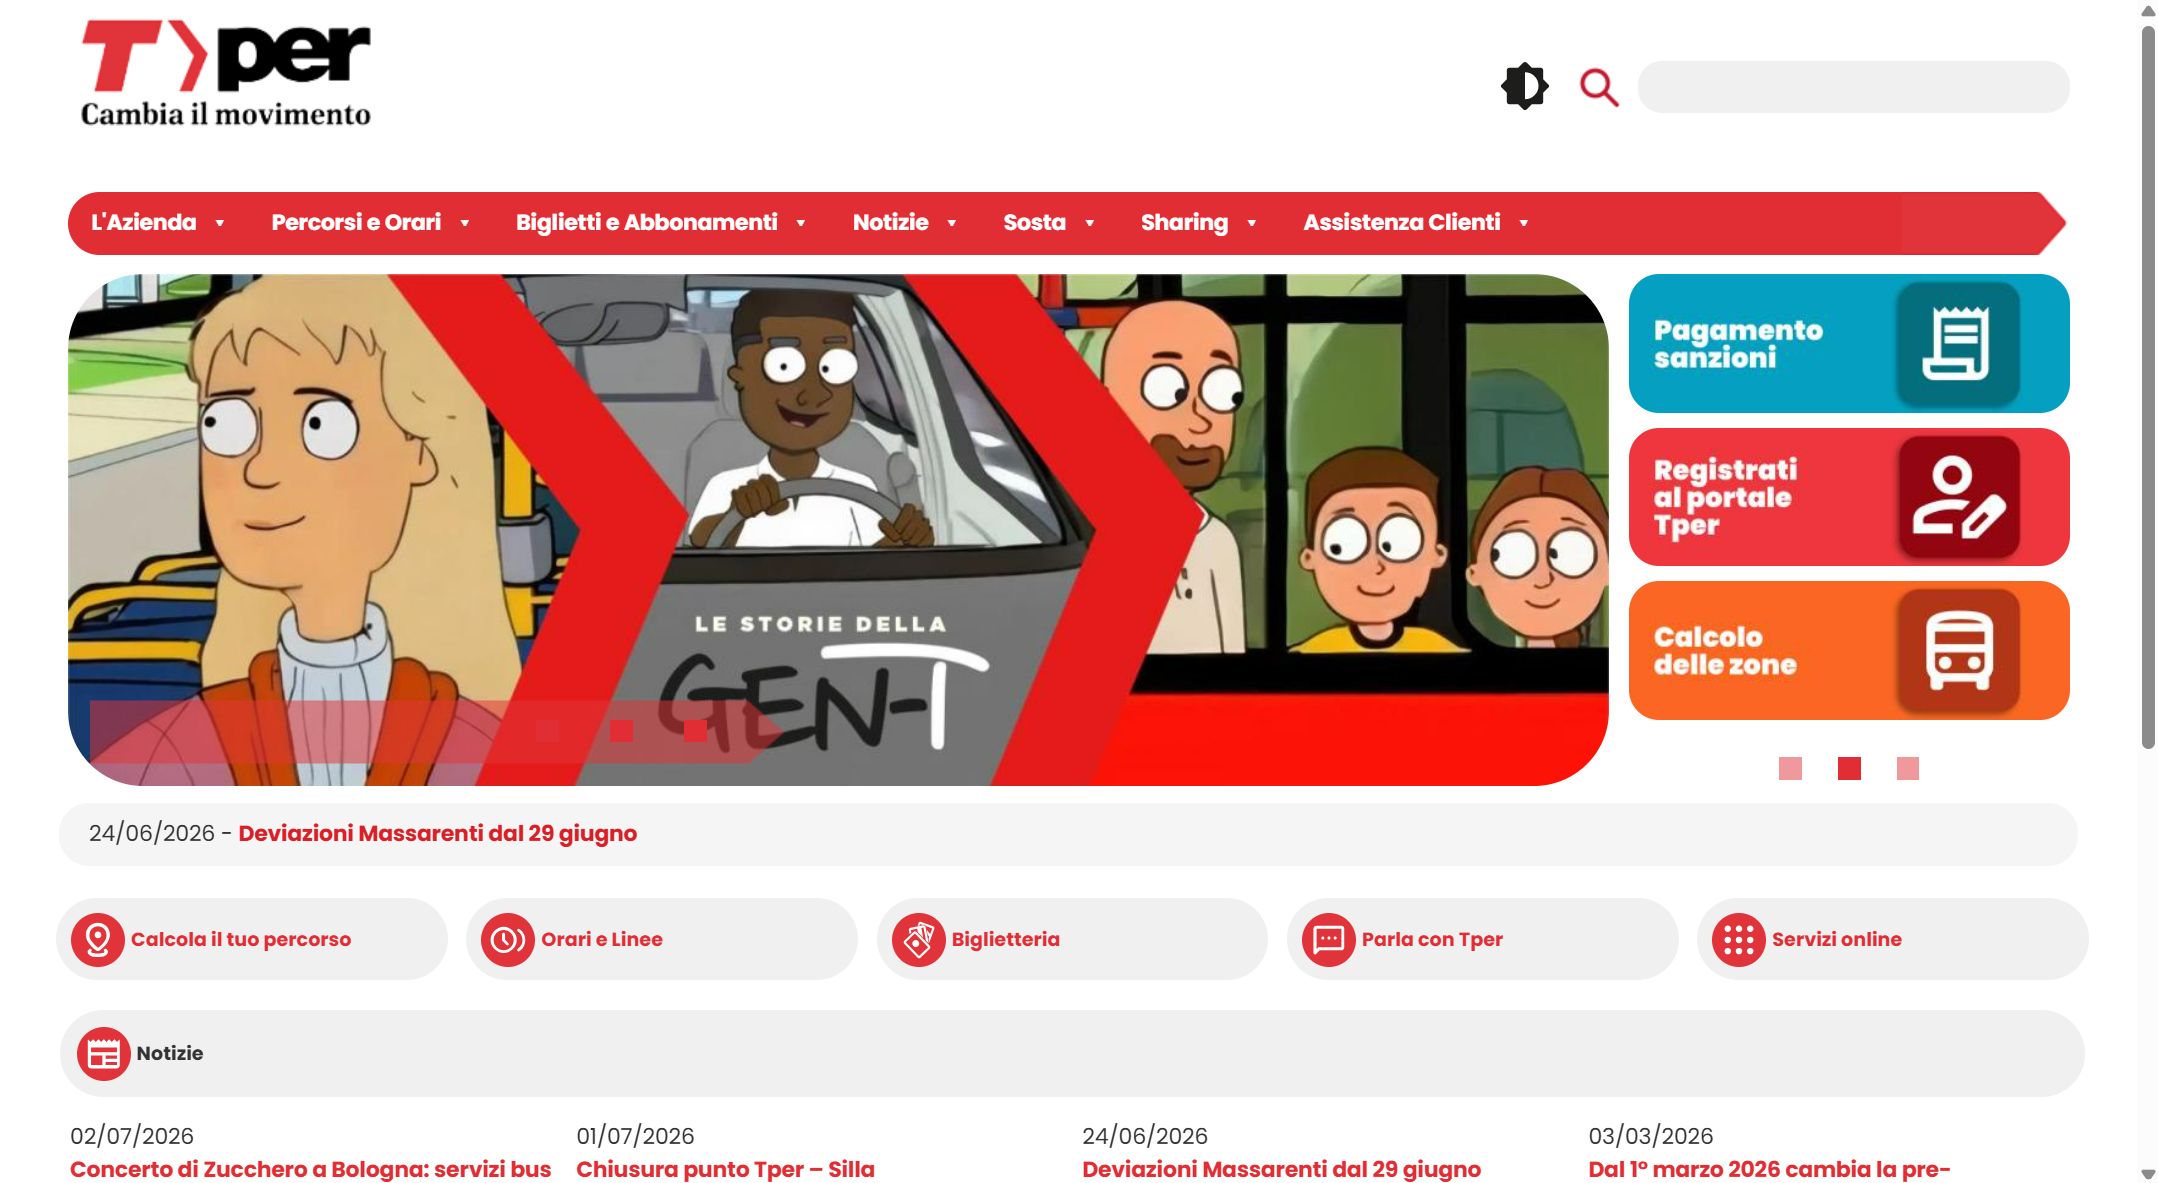
\includegraphics[width=0.85\textwidth]{Tper sito originale/Homepage.png}
\par\small\textit{Before: \texttt{tper.it} live --- corporate news slider, no primary CTA}
\vspace{0.4cm}
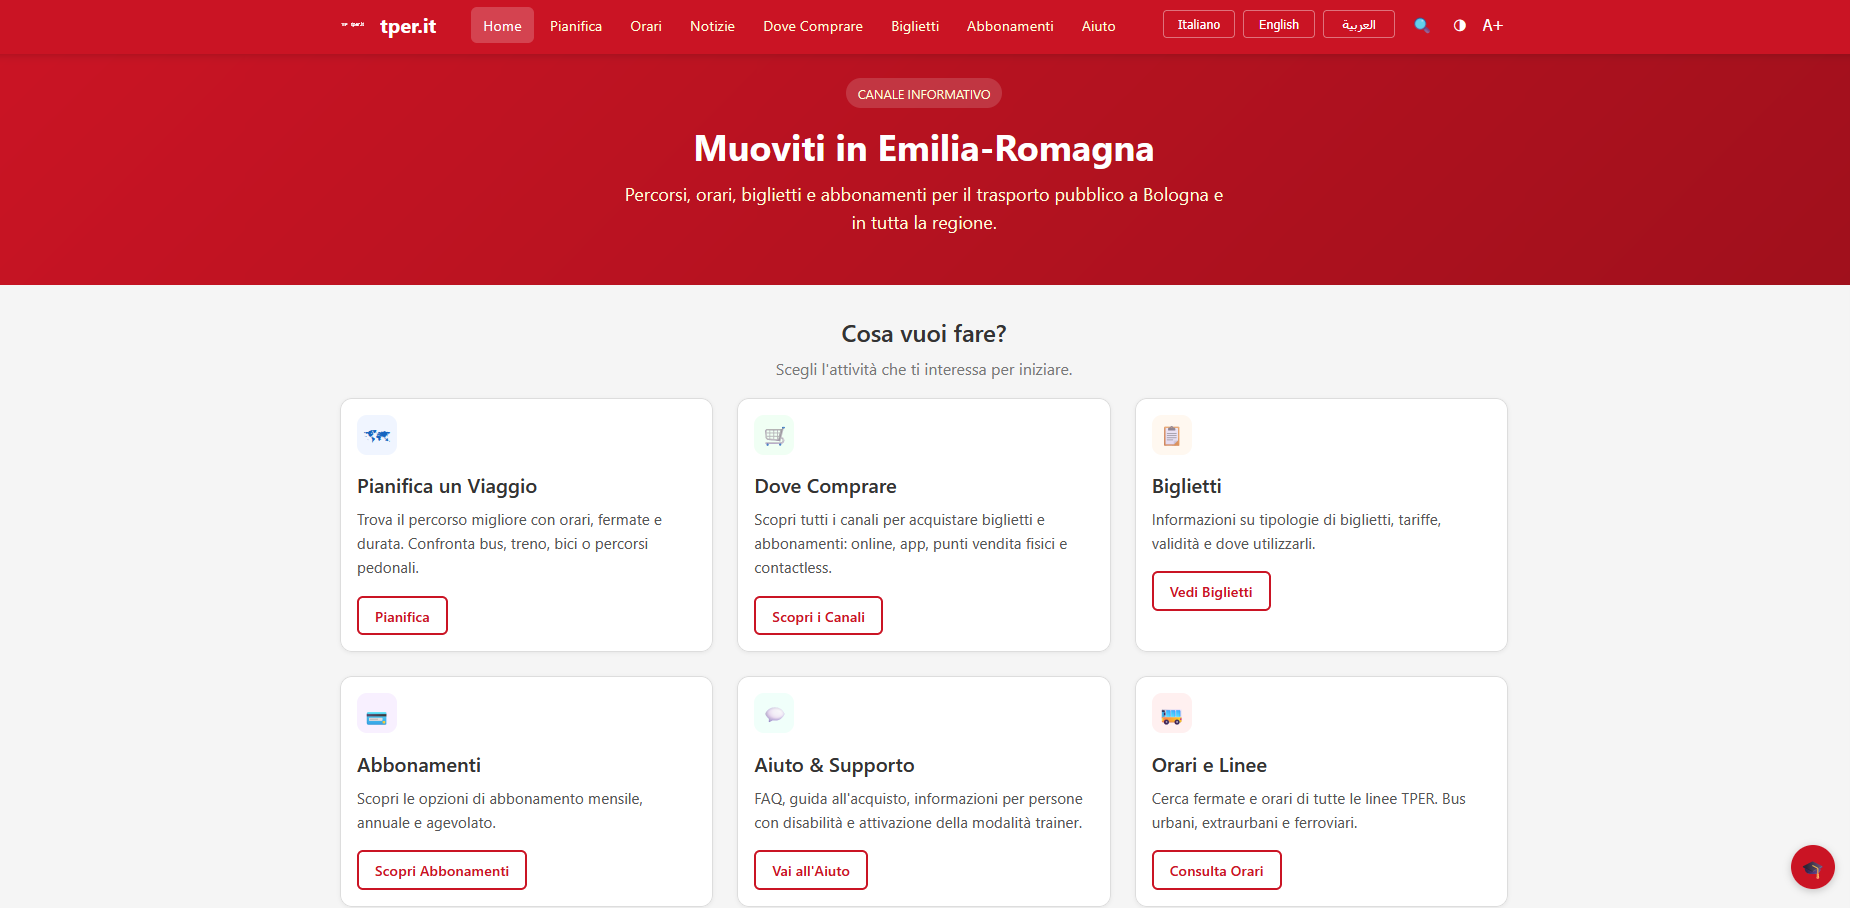
\includegraphics[width=0.85\textwidth]{Redesign Tper 2.0/homepage.png}
\par\small\textit{After: tper 2.0 --- hero route planner + 6 task-oriented cards grid}
\caption{\texttt{tper.it} Homepage}
\label{fig:comparison-home}
\end{figure}

\begin{table}[H]
\centering
\small
\renewcommand{\arraystretch}{1.4}
\begin{tabular}{|p{0.5cm}|p{7cm}|p{7cm}|}
\hline
& \textbf{Before} & \textbf{After} \\ \hline
\cellcolor{primaryColor!15} &
\textit{Current \texttt{tper.it} homepage (live)} &
\textit{\texttt{tper 2.0} redesign homepage} \\ \hline

\raisebox{0.5cm}{\rotatebox{90}{\textbf{Content}}} &
Corporate news slider, press releases, tender notices occupy the homepage. The trip planner is reachable after 2--3 clicks through \textit{Routes and Timetables} $\rightarrow$ \textit{Calculate your route}. No hierarchy between user content and institutional content (Issue D1). &
Hero section dedicated to the trip planner with ``From'' and ``To'' fields already visible. ``What do you want to do?'' grid with 6 task-oriented cards: Plan, Where to Buy, Tickets, Subscriptions, Help, Timetables. Corporate news moved to a separate section (R1). \\ \hline

\raisebox{0.5cm}{\rotatebox{90}{\textbf{CTAs}}} &
Generic text links: ``Online Services'', ``Routes and Timetables'', ``Ticketing'', ``Talk to Tper''. The user must interpret corporate terminology to understand where to go (Issue D3). &
Large buttons with icons and user language: ``Plan a Trip'', ``Where to Buy?'', ``View Tickets'', ``Discover Subscriptions'', ``Go to Help'', ``Check Timetables''. Each card shows a distinctive coloured icon (R2, R9). \\ \hline

\raisebox{0.5cm}{\rotatebox{90}{\textbf{Navigation}}} &
Mega-menu with 7 main items and over 50 sub-items, dominated by institutional content: \textit{Transparent Company}, \textit{Procurement and Suppliers}, \textit{The Company} occupy most of the space. The user gets lost among legal content (Issue D2). &
Flat navigation with 8 task-oriented items: Home, Plan, Timetables, News, \textbf{Where to Buy}, Tickets, Subscriptions, Help. Breadcrumb on all internal pages for orientation. Institutional content available via footer (R2, R3). \\ \hline

\raisebox{0.5cm}{\rotatebox{90}{\textbf{Info}}} &
No indication of the site's informational role. The user searches for transactional functions that do not exist on \texttt{tper.it} (UR-01, UR-03). &
Explicit banner on every page: ``\texttt{tper.it} is an informational website. To purchase tickets and subscriptions please use one of the dedicated channels'' with a link to Where to Buy. Hero badge: ``INFORMATIONAL CHANNEL'' (R1). \\ \hline
\end{tabular}
\caption{Homepage (\texttt{tper.it} live vs tper 2.0)}
\label{tab:comparison-home}
\end{table}

\vspace{0.3cm}

% ============================================================
% COMPARISON 2: solweb HOMEPAGE
% ============================================================
\section{\texttt{solweb.tper.it} Home Page}
\label{sec:comparison-solweb-home}

\textbf{D5 $\rightarrow$ R7} --- Mandatory login (P3,I5) $\rightarrow$ Guest path + 4 quick actions. 3/4 failed T3, unsignalled \texttt{tper.it}$\rightarrow$\texttt{solweb} transition.

\begin{figure}[H]
\centering
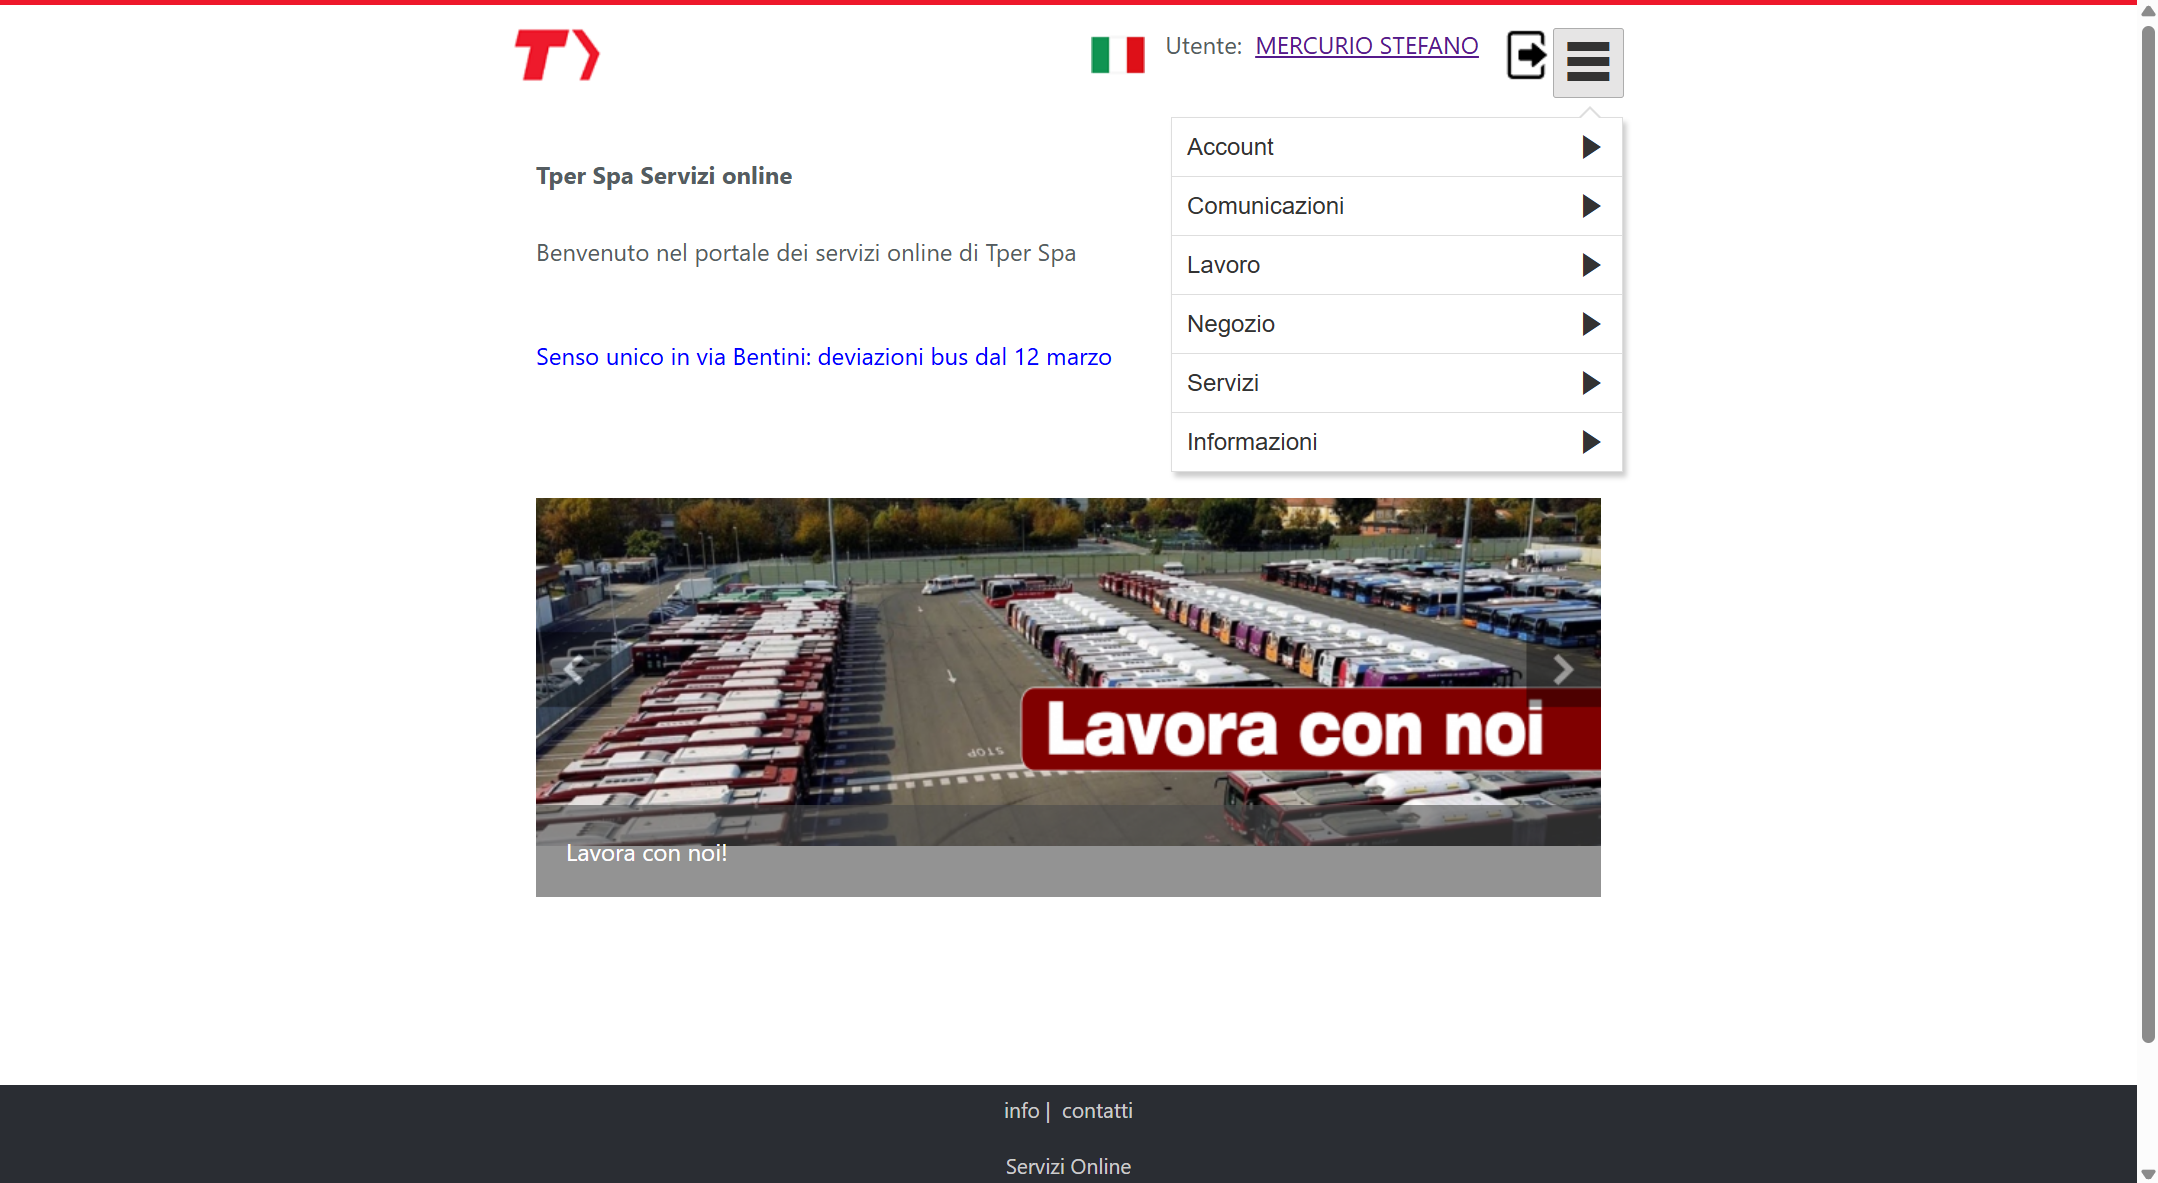
\includegraphics[width=0.85\textwidth]{Tper sito originale/HomepageS.png}\\[2pt]
{\small\textit{+ second view:}}\\[2pt]
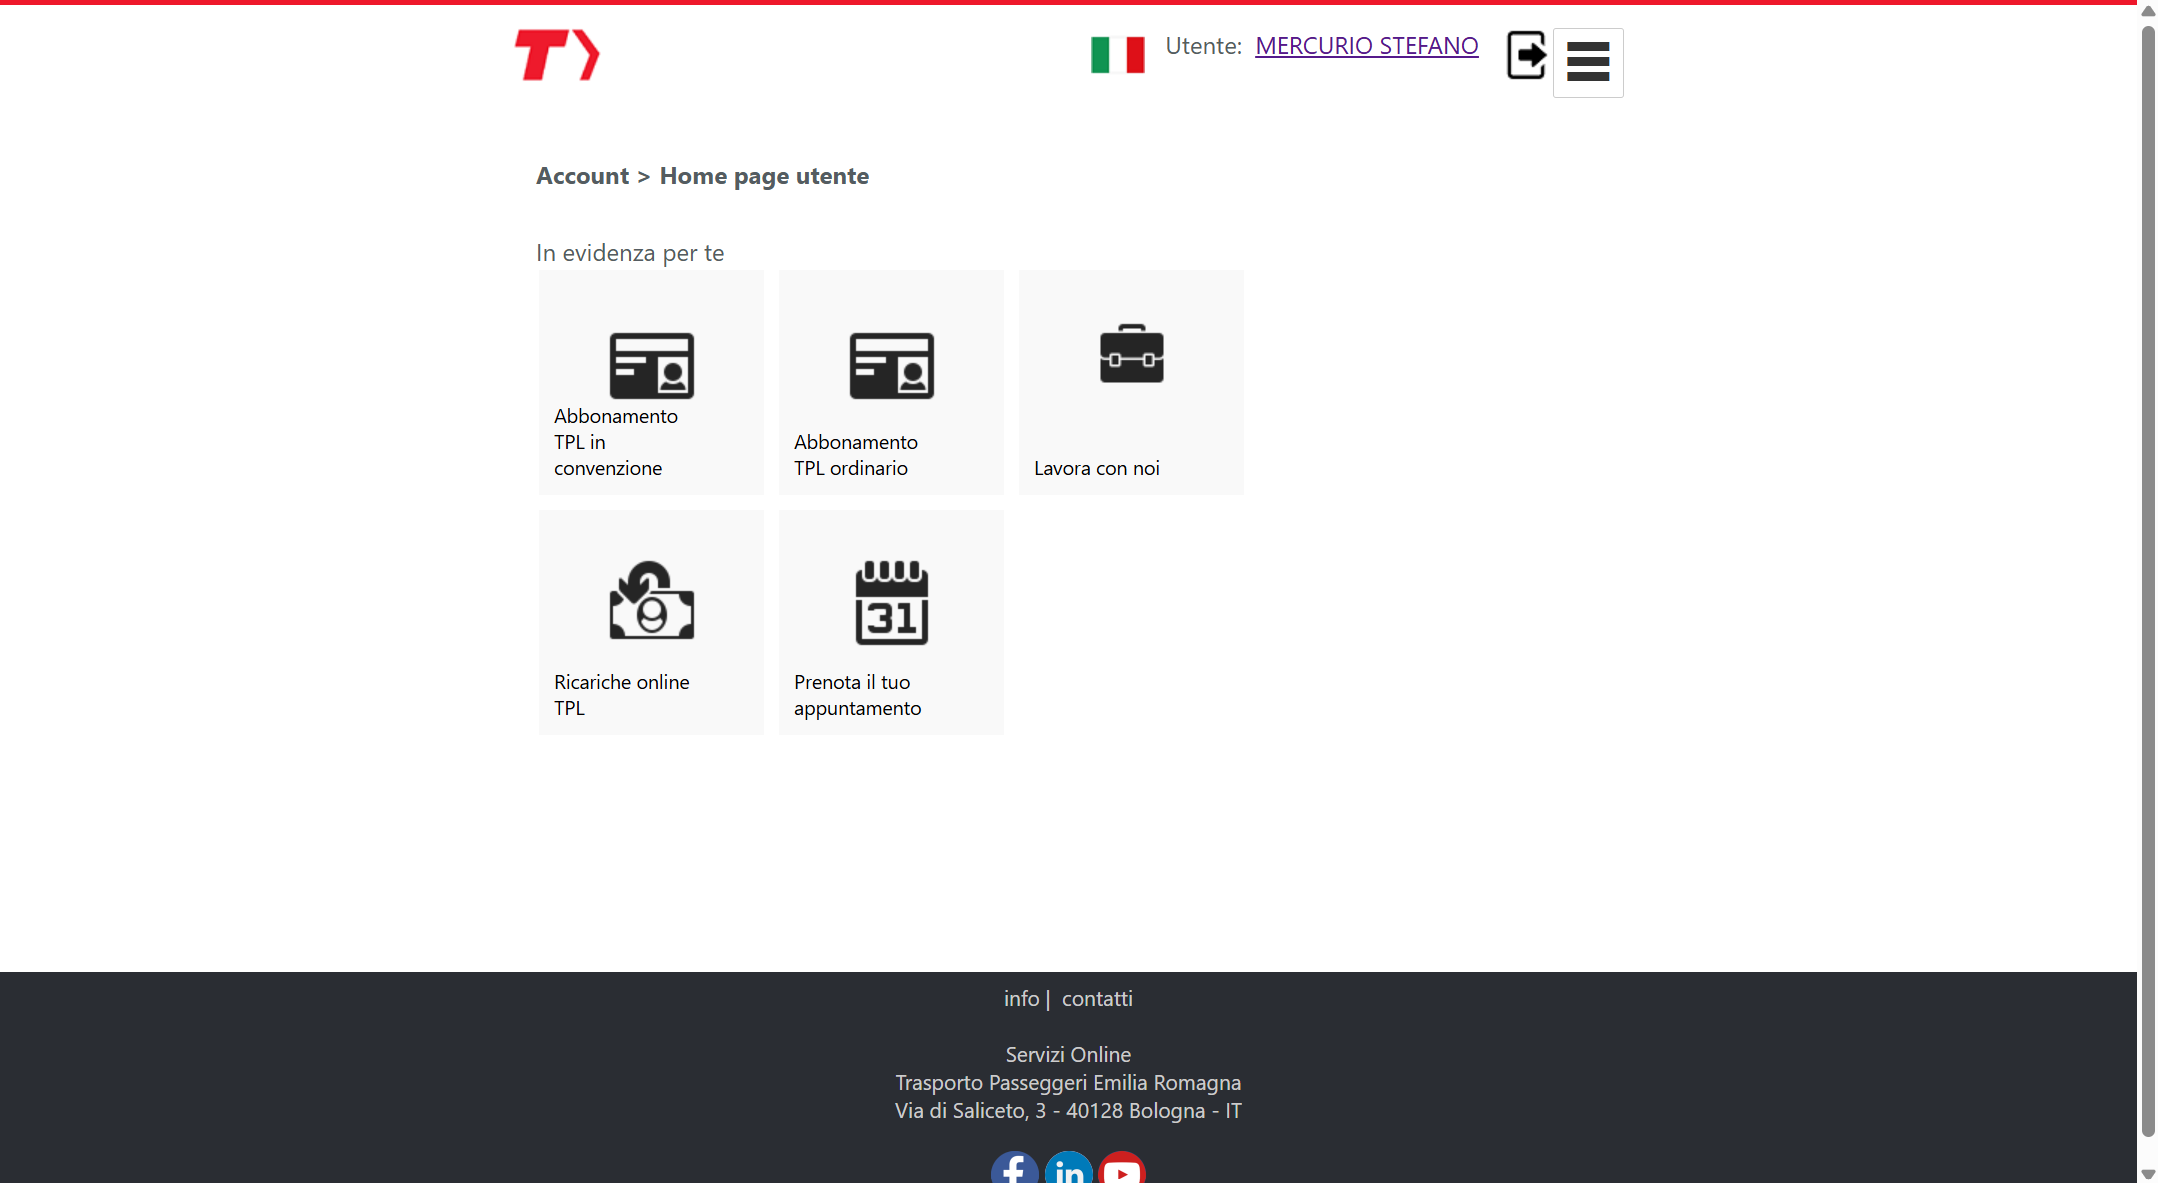
\includegraphics[width=0.85\textwidth]{Tper sito originale/HomepageS2.png}
\par\small\textit{Before: original \texttt{solweb} --- mandatory login, no guest path}
\vspace{0.4cm}
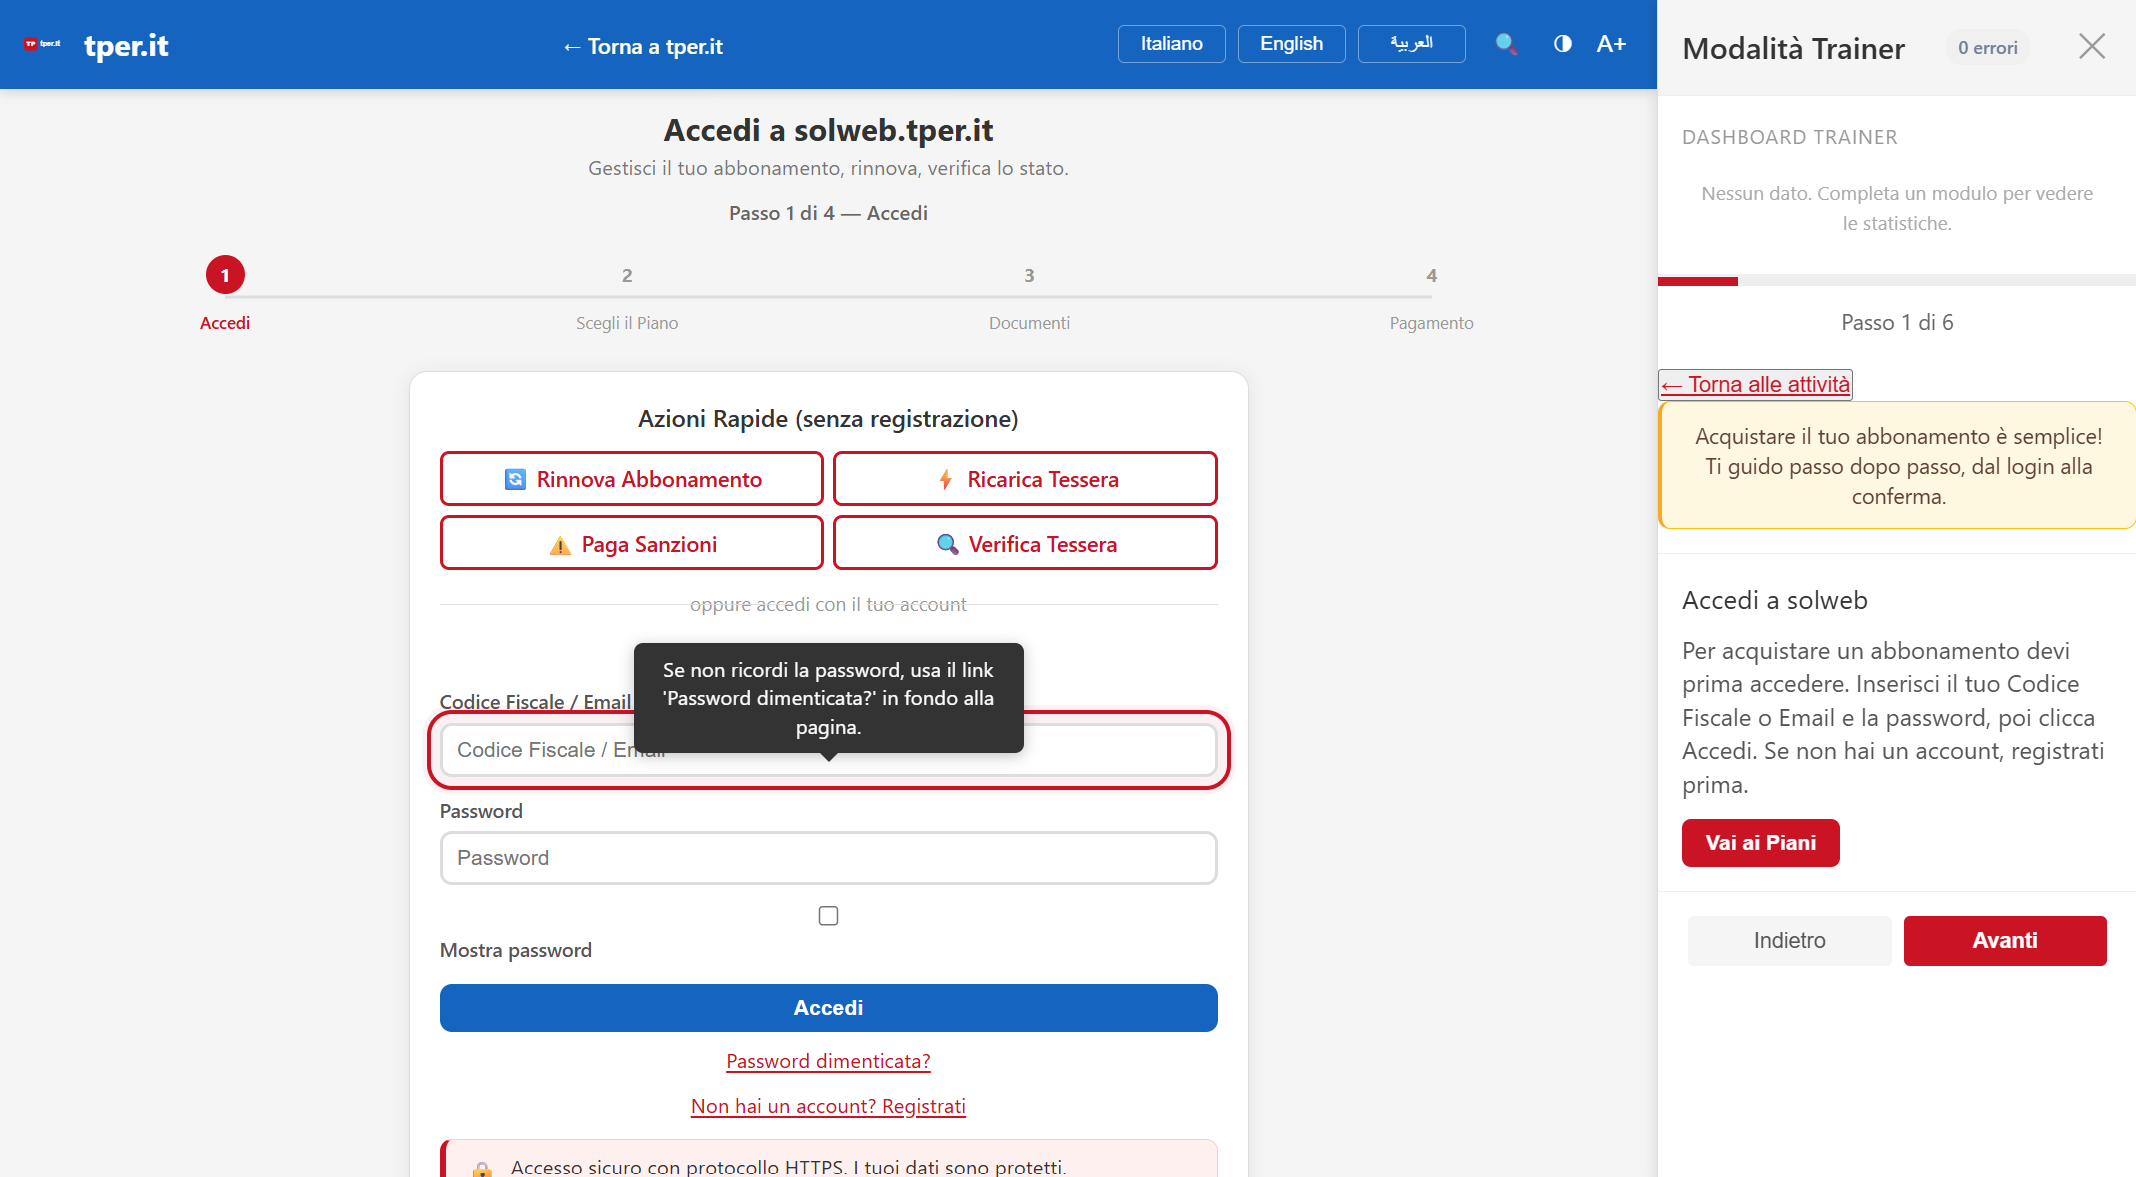
\includegraphics[width=0.85\textwidth]{Redesign Tper 2.0/HomepageS.png}
\par\small\textit{After: solweb 2.0 --- login + 4 quick actions without registration}
\caption{\texttt{solweb.tper.it} Homepage}
\label{fig:comparison-solweb-home}
\end{figure}

\begin{table}[H]
\centering
\small
\renewcommand{\arraystretch}{1.4}
\begin{tabular}{|p{0.5cm}|p{7cm}|p{7cm}|}
\hline
& \textbf{Before} & \textbf{After} \\ \hline
\cellcolor{primaryColor!15} &
\textit{Original solweb portal} &
\textit{solweb 2.0 in the redesign} \\ \hline

\raisebox{0.5cm}{\rotatebox{90}{\textbf{Access}}} &
\textbf{Login only}: username/SPID/CIE required for any operation. No guest alternative. For an elderly user with low digital competence, the mere request to ``create an account'' causes immediate abandonment (Issue D5). &
\textbf{4 quick actions without login}: Impersonal Renewal, Card Top-up, Pay Fines, Verify Card. Login remains available for operations requiring authentication (ISEE, personal subscriptions). 4-step progress bar: Login $\rightarrow$ Choose Plan $\rightarrow$ Documents $\rightarrow$ Payment (R7). \\ \hline

\raisebox{0.5cm}{\rotatebox{90}{\textbf{Transition}}} &
Switch from \texttt{tper.it} to \texttt{solweb} with no warning: domain, interface, colours, and layout all change. The user does not know if they are still on TPER (Issue R4). &
\textbf{Transition modal} before every external link: ``You are about to leave \texttt{tper.it} --- You will be redirected to the external purchase channel'' with the destination URL visible (R9). Solweb header with ``$\leftarrow$ Back to tper.it'' link always visible. \\ \hline

\raisebox{0.5cm}{\rotatebox{90}{\textbf{Orientation}}} &
No indication of where one is within the ecosystem. Interface completely different from \texttt{tper.it}, zero continuity signage. &
Blue header (\#1565C0) distinct from TPER red to signal the platform change. Hero badge ``SUBSCRIPTION PLATFORM'' in the dashboard. Contextual breadcrumbs. \\ \hline

\raisebox{0.5cm}{\rotatebox{90}{\textbf{Operations}}} &
All operations require registration. No distinction between simple operations (top-up, fines) and complex ones (ISEE, personal renewal). &
\textbf{Guest/authenticated separation}: top-up, fines, and card verification accessible without login. Purchase and personal renewal protected by authentication with an explanation of why this is needed (R7). \\ \hline
\end{tabular}
\caption{\texttt{solweb.tper.it} Homepage}
\label{tab:comparison-solweb-home}
\end{table}

\vspace{0.3cm}

% ============================================================
% COMPARISON 3: IA RESTRUCTURING (3v3)
% ============================================================
\section{Information Architecture Restructuring}
\label{sec:comparison-ia-3v3}

\textbf{D2+D3 $\rightarrow$ R2+R9} --- 200+ items, 5 levels $\rightarrow$ Flat nav 8 items. ``Sales Network'' buried 3 levels deep.

\subsection*{The Original Problem}

In the original site, Tickets, Subscriptions, and Tariffs were not three separate pages but \textbf{three sections of the same page}, creating information overload:

\begin{itemize}[nosep]
    \item \textbf{Tickets}: listed tickets + sales channels + tariffs --- too many functions in a single page;
    \item \textbf{Subscriptions}: listed subscriptions + channels + tariffs --- the same duplication as the Tickets section;
    \item \textbf{Tariffs}: a pricing section on the same page, \textbf{redundant} and disconnected from the usage context.
\end{itemize}

Result: the user had to \textbf{scroll through a single page} visually comparing different sections to answer questions like \textit{``which subscription should I buy?''} and \textit{``where do I buy it?''}. The channel guide (``Sales Network'') was buried three navigation levels deep.

\subsection*{The Solution: Separation of Concerns}

The redesign applies the \textbf{one page, one task} principle (R2), eliminating all duplication:

\begin{itemize}[nosep]
    \item \textbf{Tickets}: \textit{only} ticket types + 5-question wizard + filters for zone/validity/channel;
    \item \textbf{Subscriptions}: \textit{only} subscription plans + 7-question wizard + concession eligibility check;
    \item \textbf{Where to Buy}: \textbf{new dedicated section} gathering all channel guidance --- 3-question wizard, 6 channel cards, comparison table 5$\times$7.
\end{itemize}

\textbf{Tariffs} have been \textbf{integrated} directly into Tickets and Subscriptions: the price appears at the exact moment of the product decision, not on a separate page.

\begin{figure}[H]
\centering
\textbf{Before --- Original Site}\\[4pt]
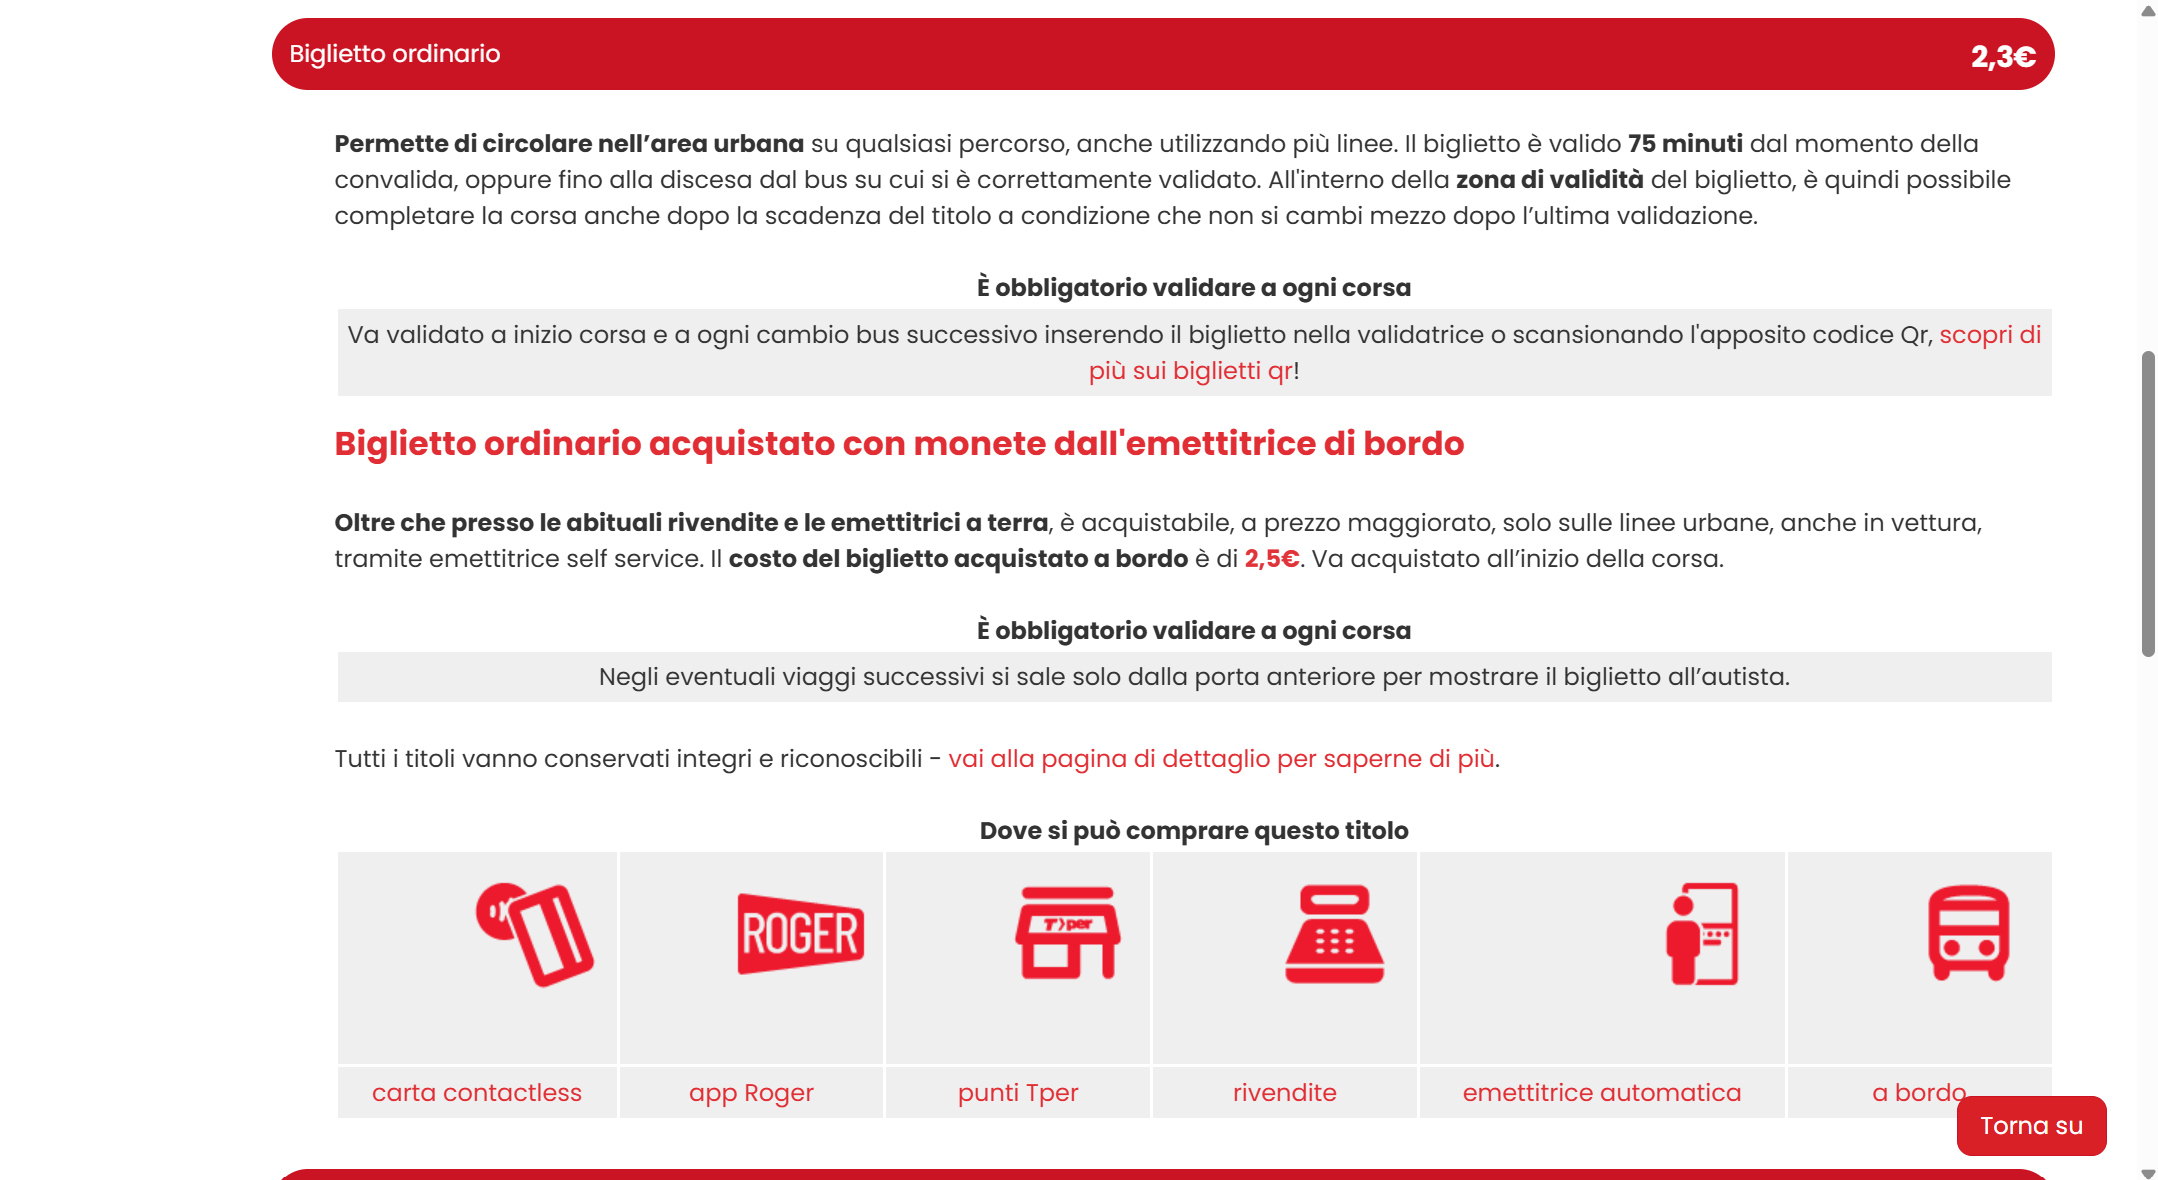
\includegraphics[width=0.332\textwidth]{Tper sito originale/Biglietti.png}\hfill
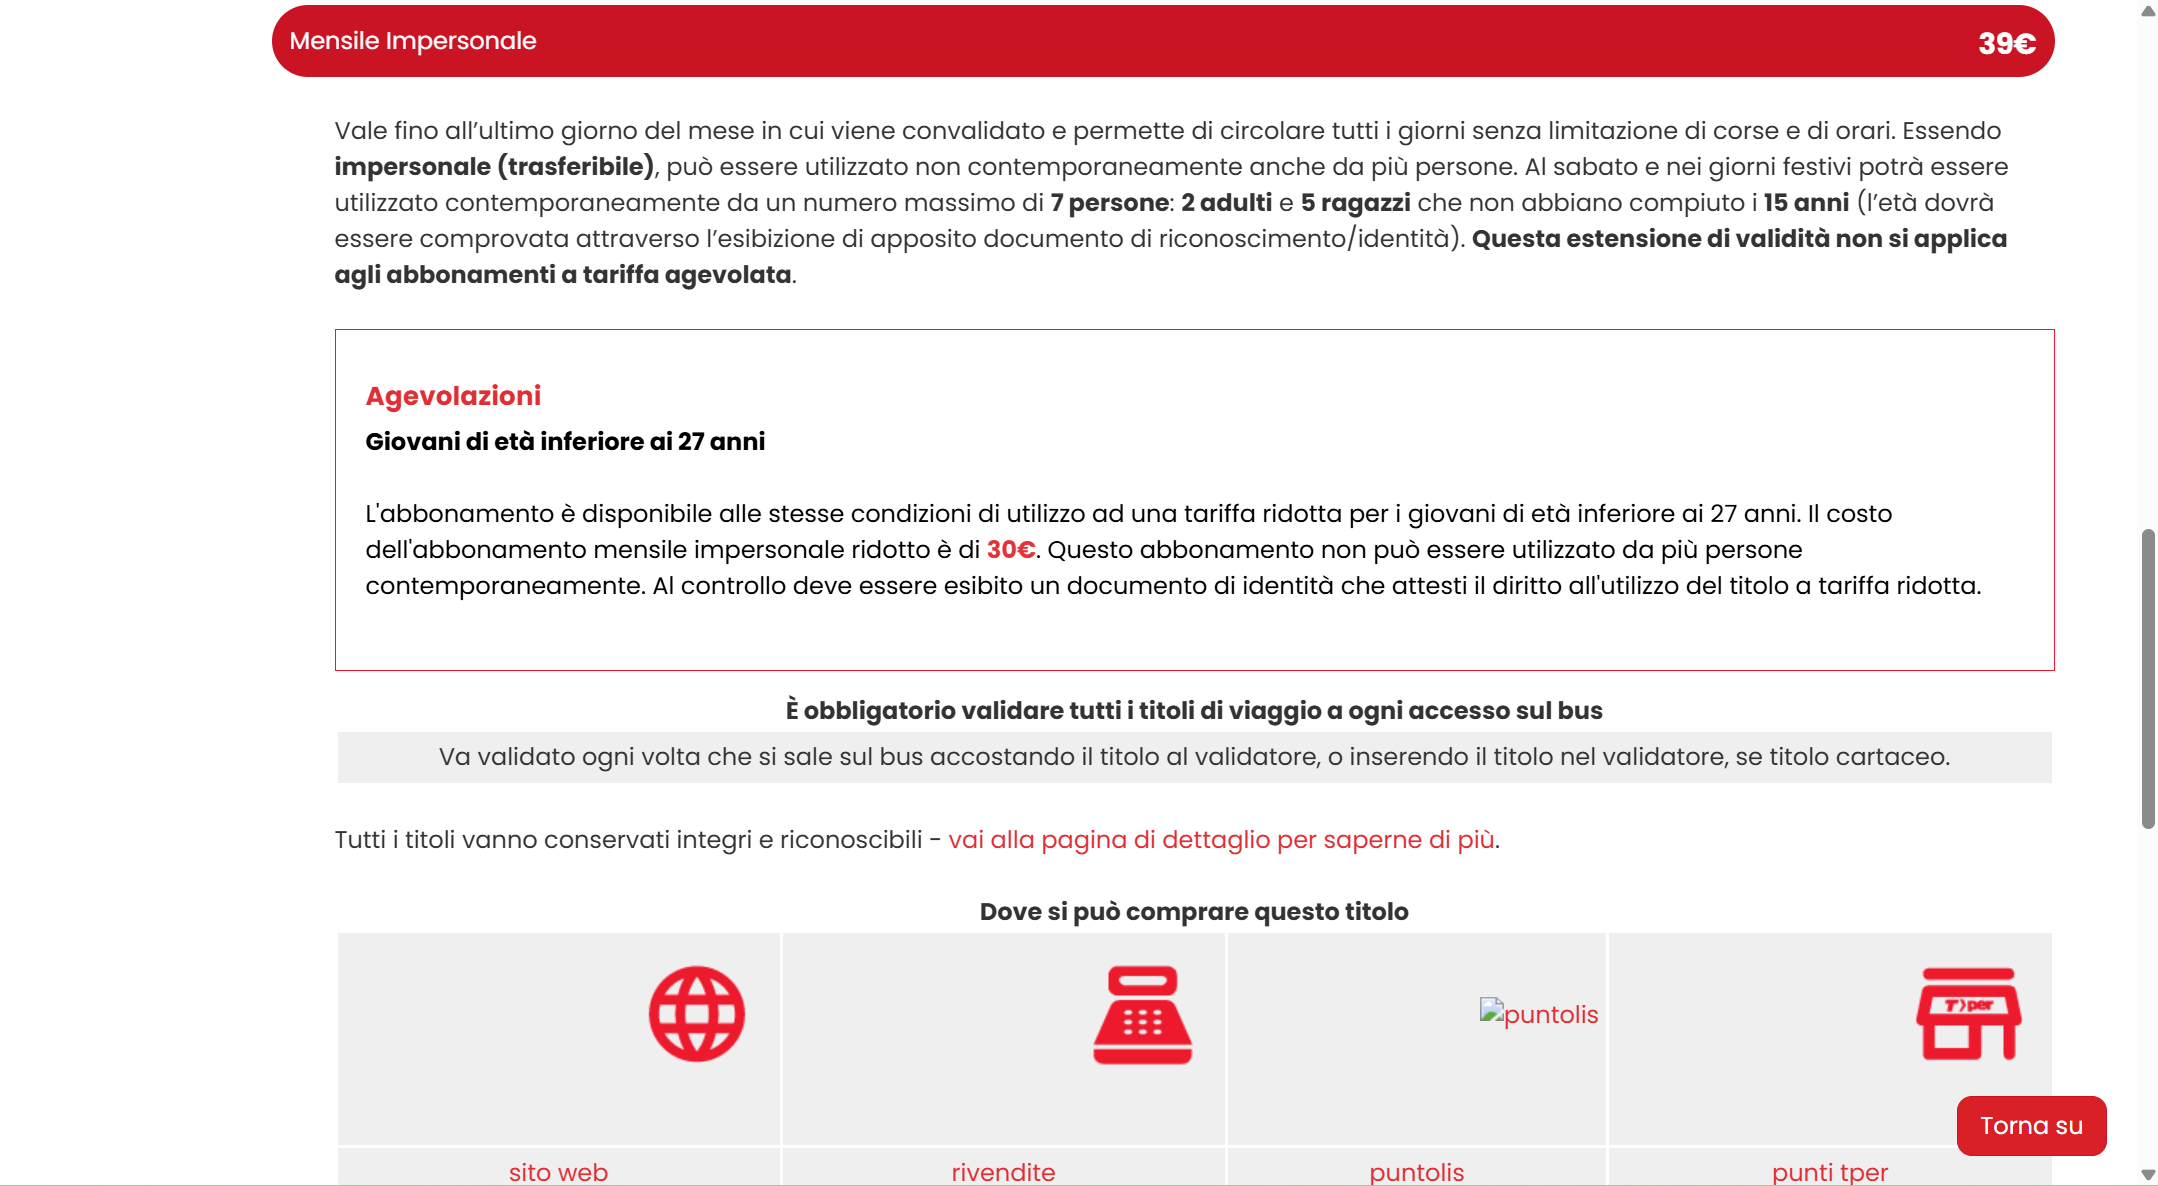
\includegraphics[width=0.332\textwidth]{Tper sito originale/Abbonamenti.png}\hfill
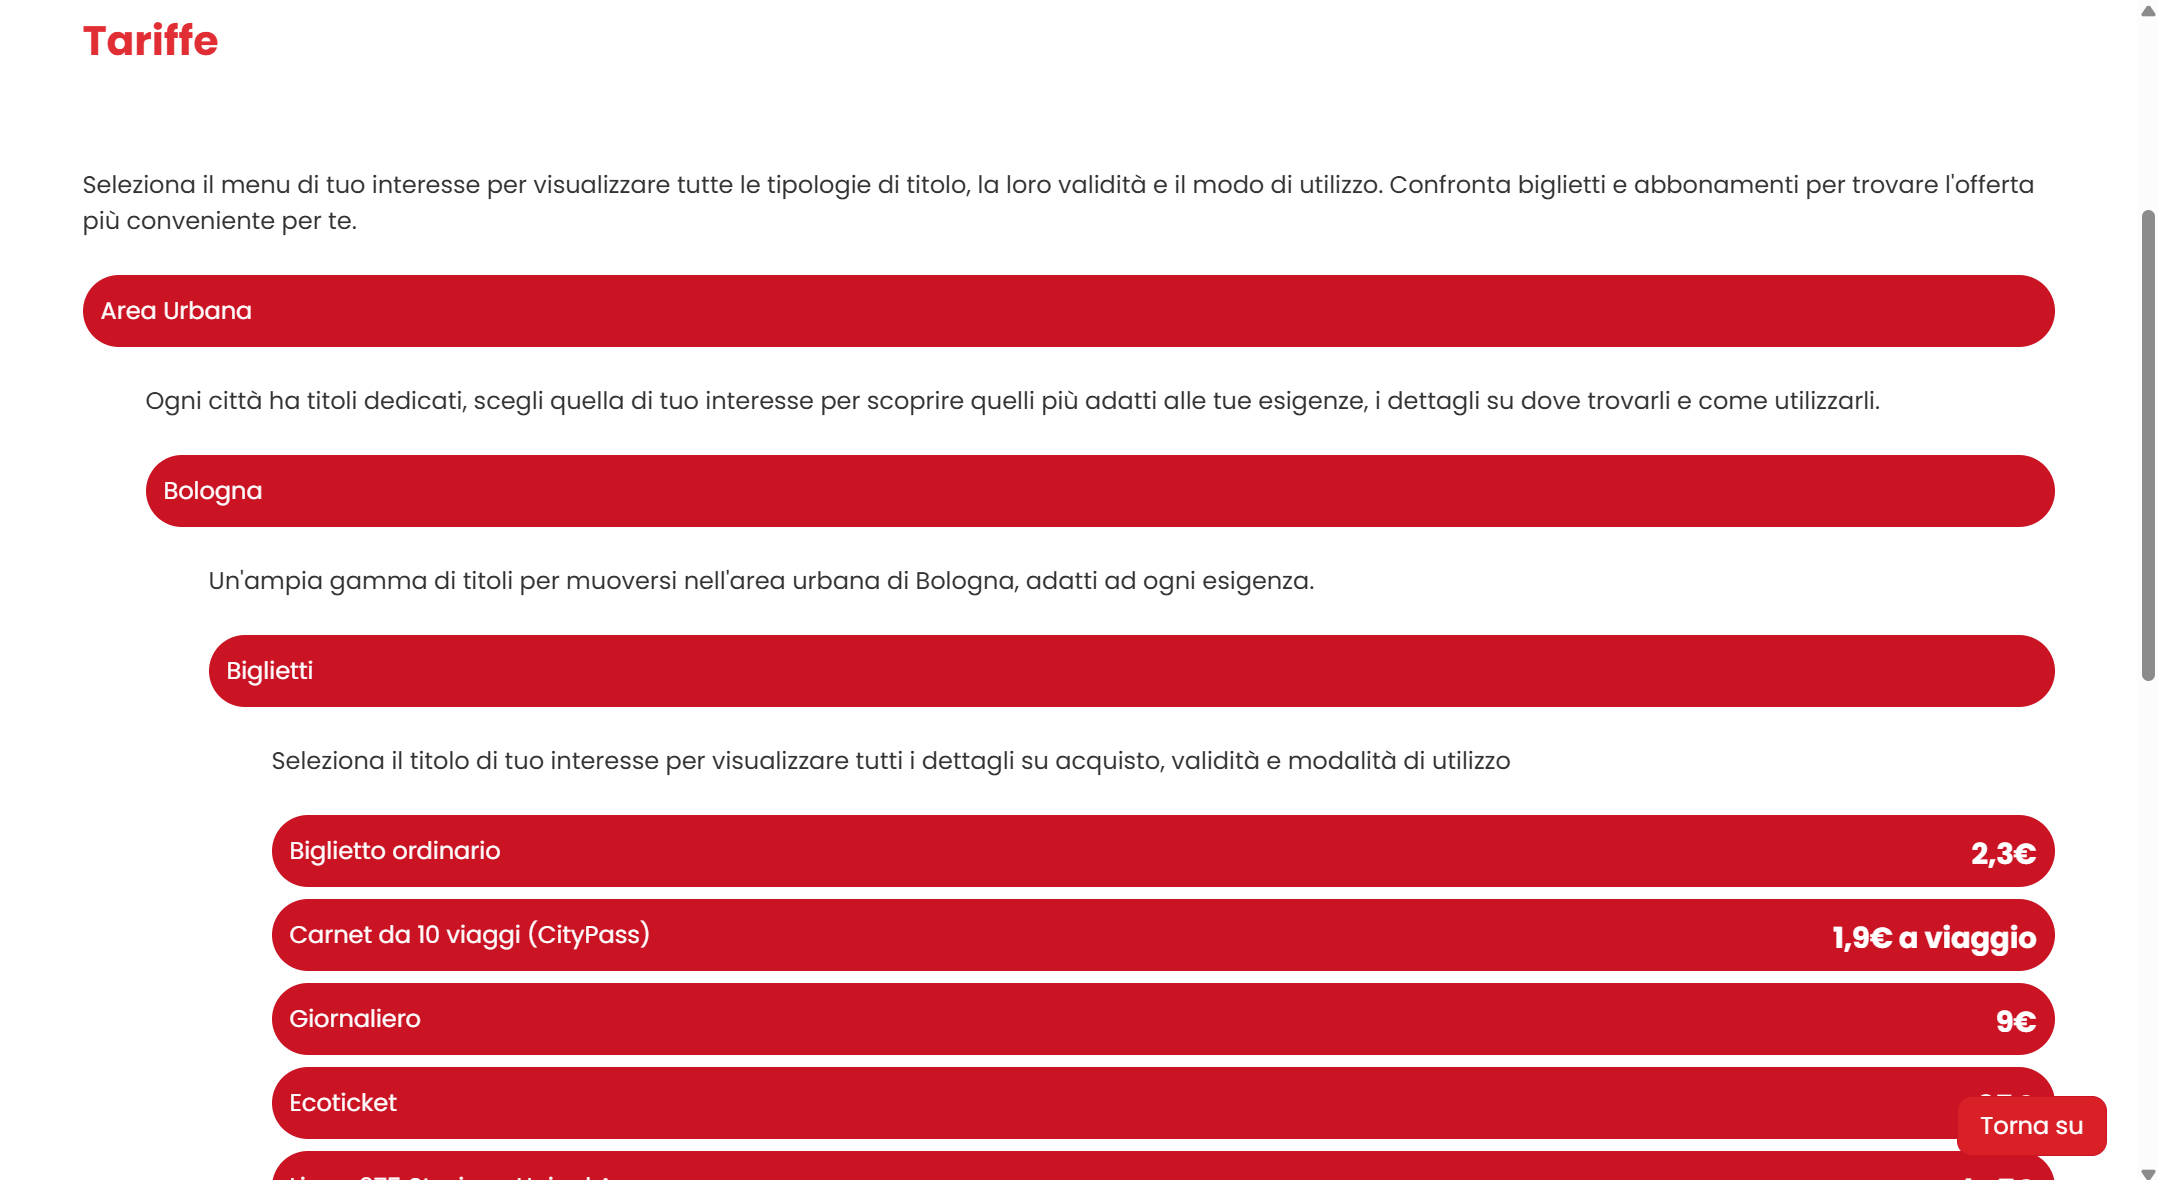
\includegraphics[width=0.332\textwidth]{Tper sito originale/Tariffe.png}\\[2pt]
{\small\textit{Tickets \hspace{3.7cm} Subscriptions \hspace{3.3cm} Tariffs}}\\[2pt]
{\footnotesize A single page with 3 sections: duplicated content, buried channels, corporate terminology}

\vspace{0.5cm}

\textbf{After --- tper 2.0 Redesign}\\[4pt]
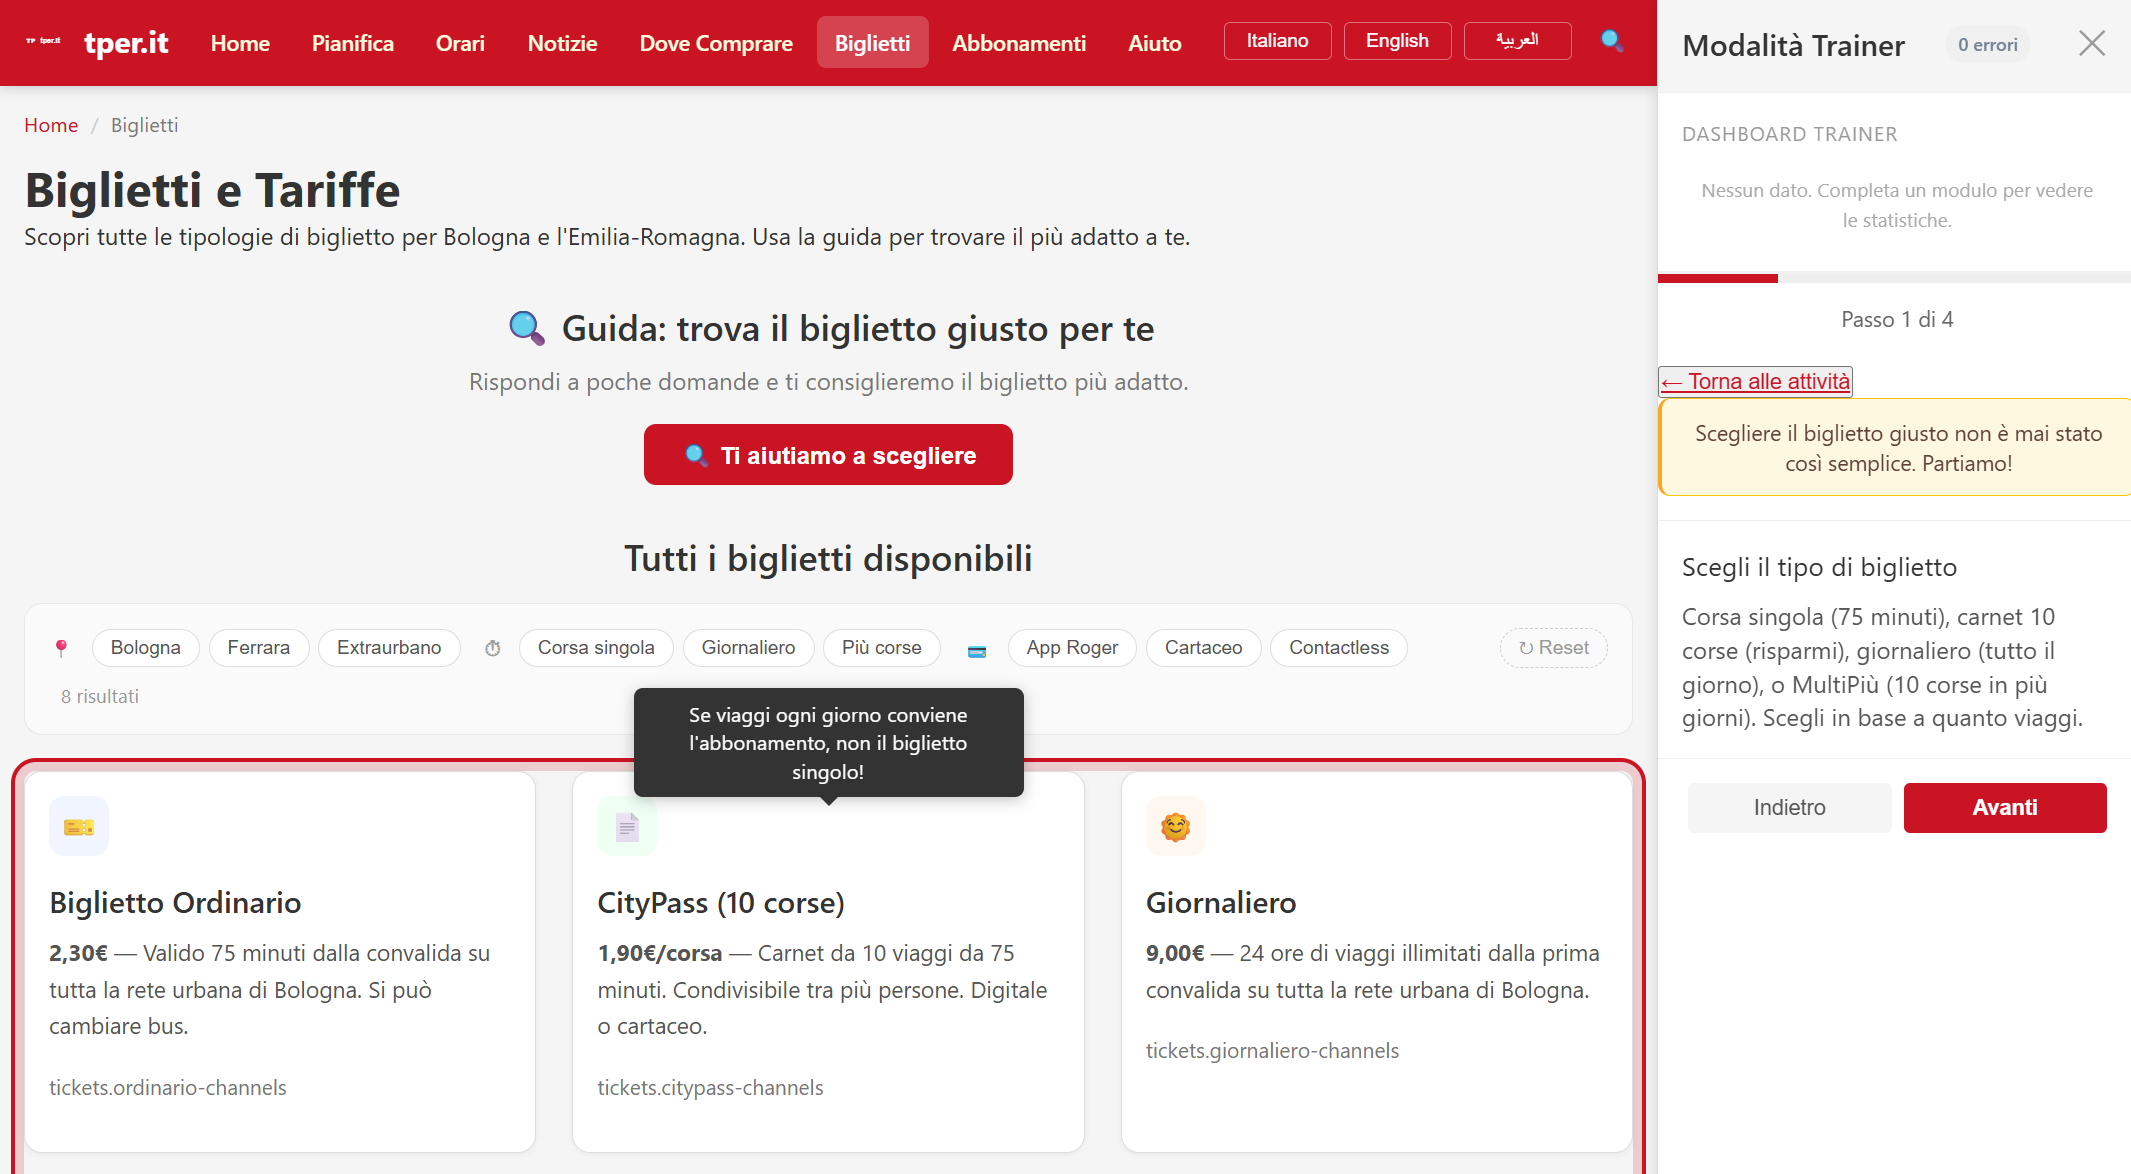
\includegraphics[width=0.332\textwidth]{Redesign Tper 2.0/Biglietti.png}\hfill
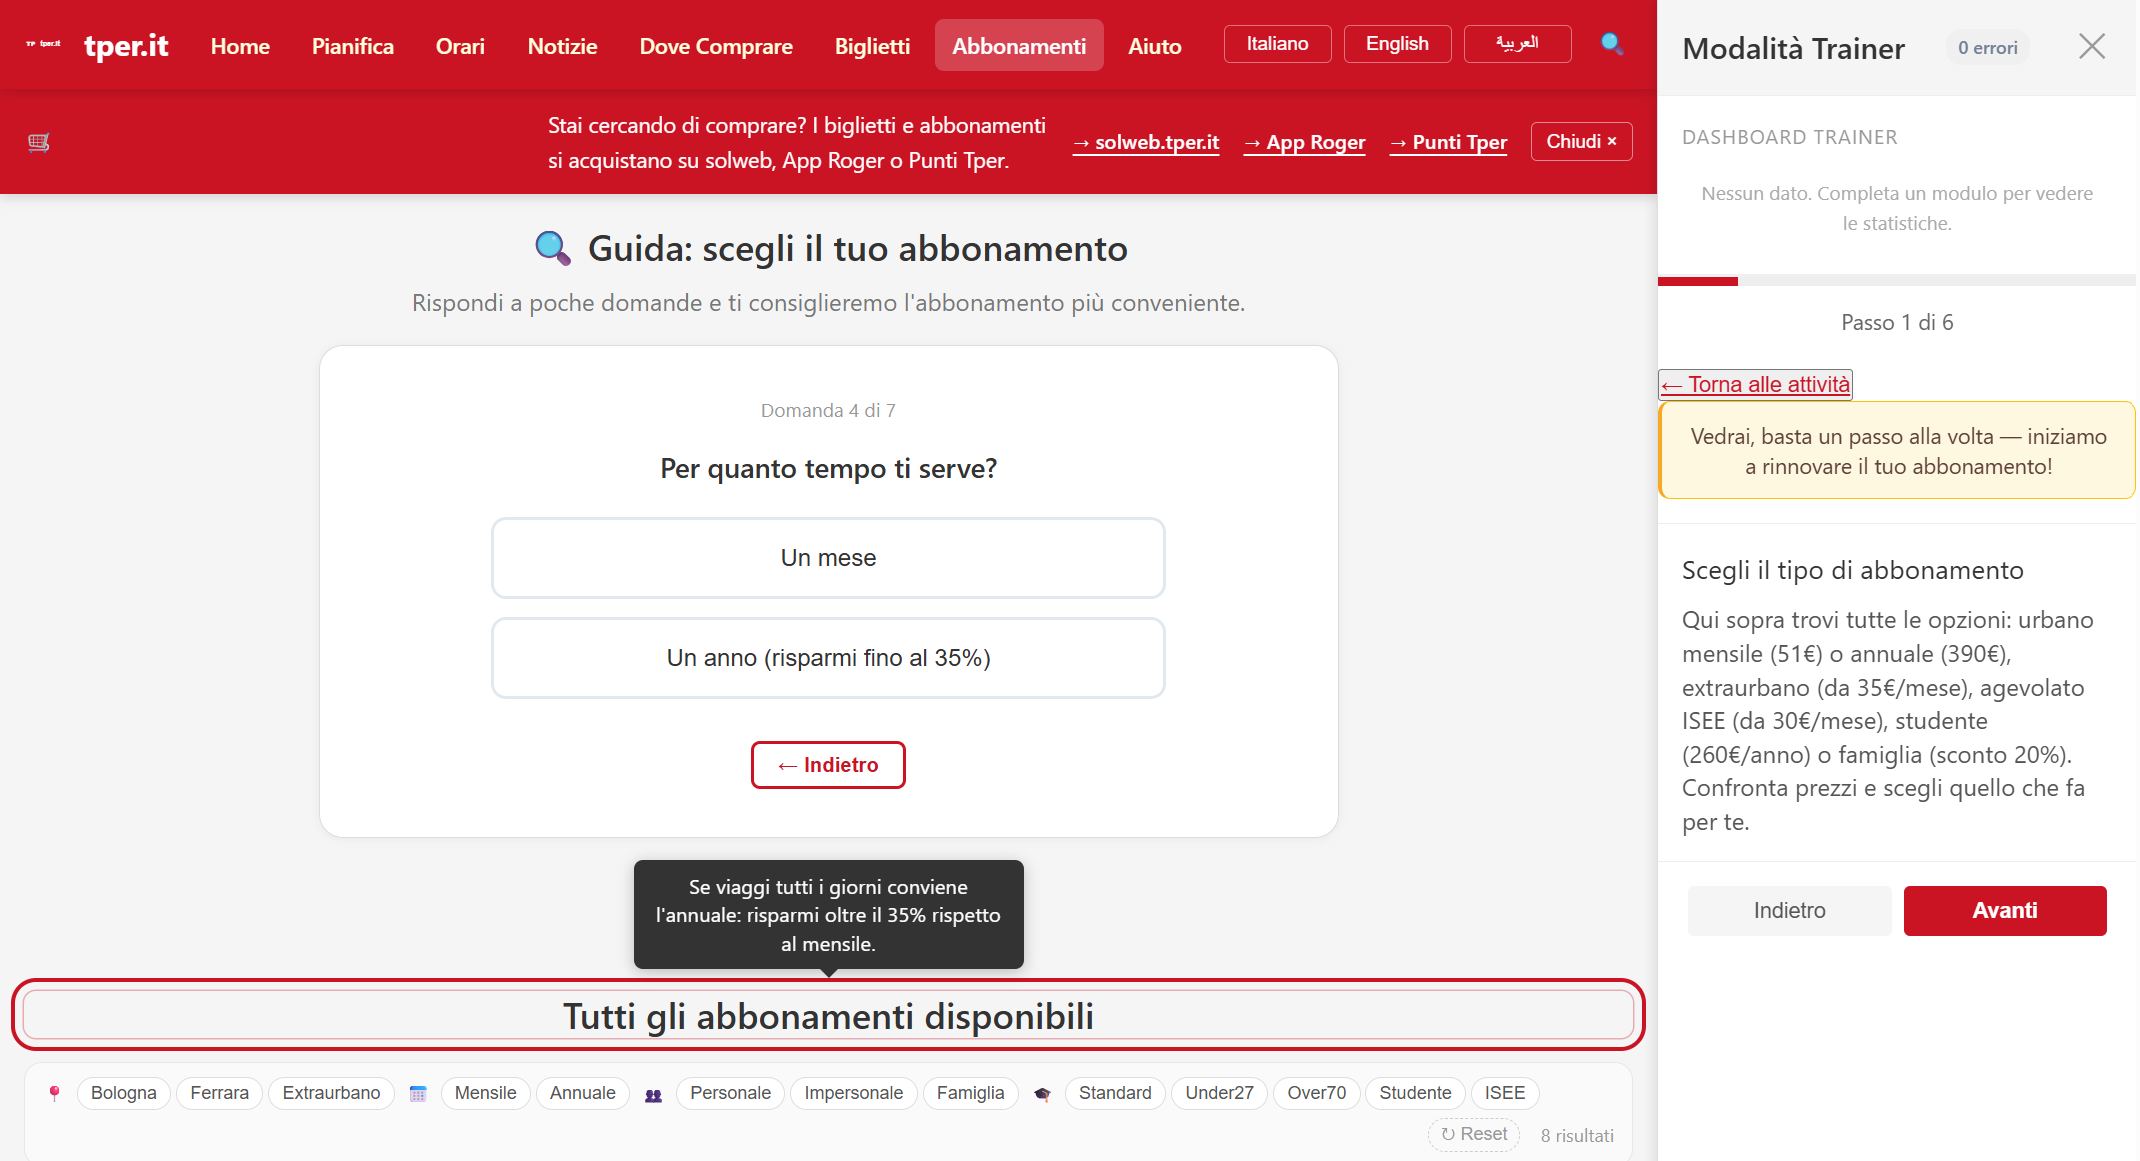
\includegraphics[width=0.332\textwidth]{Redesign Tper 2.0/Abbonamenti.png}\hfill
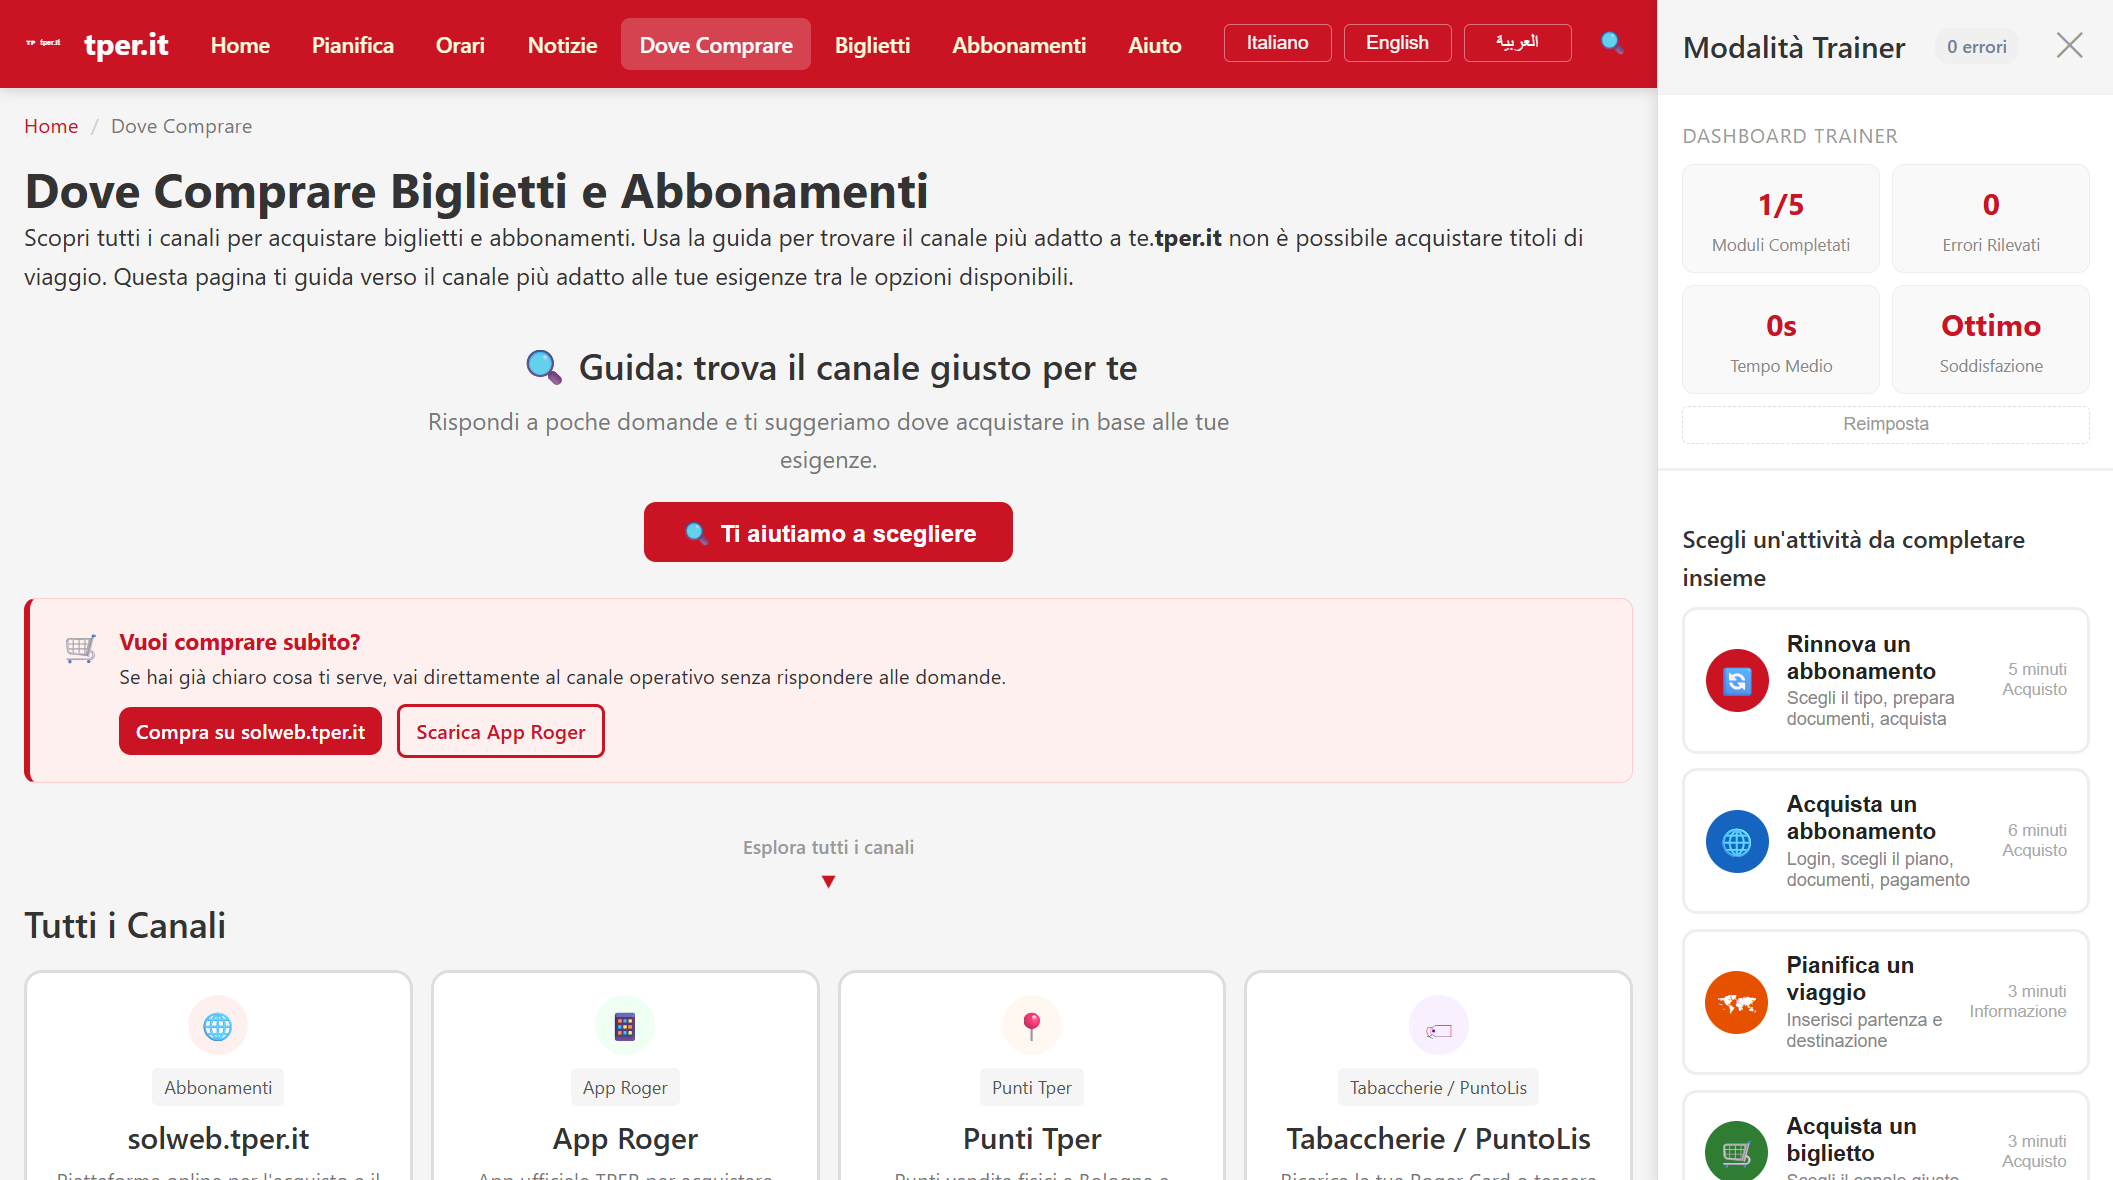
\includegraphics[width=0.332\textwidth]{Redesign Tper 2.0/Dove Comprare.png}\\[2pt]
{\small\textit{Tickets \hspace{3.7cm} Subscriptions \hspace{2.8cm} Where to Buy}}\\[2pt]
{\footnotesize 3 specialised pages: each page has a unique task, tariffs integrated into products}

\caption{3v3 Comparison --- Information Architecture Restructuring}
\label{fig:comparison-ia-3v3}
\end{figure}

\begin{table}[H]
\centering
\small
\renewcommand{\arraystretch}{1.4}
\begin{tabular}{|p{0.5cm}|p{7cm}|p{7cm}|}
\hline
& \textbf{Before (Original)} & \textbf{After (Redesign 2.0)} \\ \hline
\cellcolor{primaryColor!15} &
\textit{A single page, 3 overlapping sections} &
\textit{3 specialised pages} \\ \hline

\raisebox{0.5cm}{\rotatebox{90}{\textbf{Structure}}} &
A single page with 3 overlapping sections and blurred boundaries. Tickets and Subscriptions both contain references to tariffs and channels. The Tariffs section is redundant. 3+ level navigation to reach the channel guide (D2). &
3 pages with clear and distinct responsibilities. Each page has a single task. No duplication. Direct access to each section from the main navigation (max 1 click). Tariffs are displayed in the product context (R2). \\ \hline

\raisebox{0.5cm}{\rotatebox{90}{\textbf{Tickets}}} &
Lists ticket types, but also includes sales channel information and tariff references. The user cannot tell if this is the right page to decide what to buy or where to buy it (D2, D3). &
Page focused exclusively on tickets. 5-question wizard (zone, frequency, duration, app, travel companion). Filter pills for zone/validity/channel with counter and reset. Info banner: ``tper.it is an informational website''. \\ \hline

\raisebox{0.5cm}{\rotatebox{90}{\textbf{Subscriptions}}} &
Lists subscription plans with corporate terminology (MiMuovo, SaltaSu, Prontobus). Includes channels and tariffs. No selection guidance: the user must read all options and deduce which one suits them (UR-05). &
Page focused exclusively on subscriptions. 7-question wizard (action, impersonal?, zone, duration, holder, concession, channel). 4-group filter. Accordion ``How to Purchase or Renew''. Callout to check discount eligibility (R9). \\ \hline

\raisebox{0.5cm}{\rotatebox{90}{\textbf{Channels / Tariffs}}} &
\textbf{Channels}: ``Sales Network'' buried under Tickets and Subscriptions, reachable in 3 clicks. \textbf{Tariffs}: separate pricing section on the same page, disconnected from the usage context --- the user must remember the price while navigating elsewhere to decide (D3). &
\textbf{Where to Buy}: standalone, prominent section in the main navigation. 3-question wizard $\rightarrow$ recommended channel with icon, description, and direct link. Comparison table 5 channels $\times$ 7 operations. \textbf{Tariffs}: integrated into Tickets and Subscriptions --- visible at the moment of decision (R2, R4). \\ \hline

\raisebox{0.5cm}{\rotatebox{90}{\textbf{Impact}}} &
6/20 tasks completed (30\%). Average SUS 37.5/100. Maria B. (79 yrs): 0/5 tasks, 652\,s avg, 13 errors per task. &
Phase D data: Laura P. 4/5 tasks (80\%), SUS 72.5 (+35 points). T4 (concessions): from 195\,s and 7 errors to 57\,s and 0 errors. Separating concerns eliminated the confusion between ``what to buy'' and ``where to buy''. \\ \hline
\end{tabular}
\caption{IA Restructuring: Tickets, Subscriptions, and Channels}
\label{tab:comparison-ia-3v3}
\end{table}

\vspace{0.3cm}



% ============================================================
% COMPARISON 4: CONCESSIONS AND DISCOUNTS
% ============================================================
\section{Concessions and Discounts}
\label{sec:comparison-agevolazioni}

\textbf{UR-05 $\rightarrow$ R9+R11} --- User does not know which discounts they are entitled to $\rightarrow$ 4-question wizard + ISEE tooltip. David Carter pays 50\euro/month for 3 months before discovering he is entitled to 30\euro.

\begin{figure}[H]
\centering
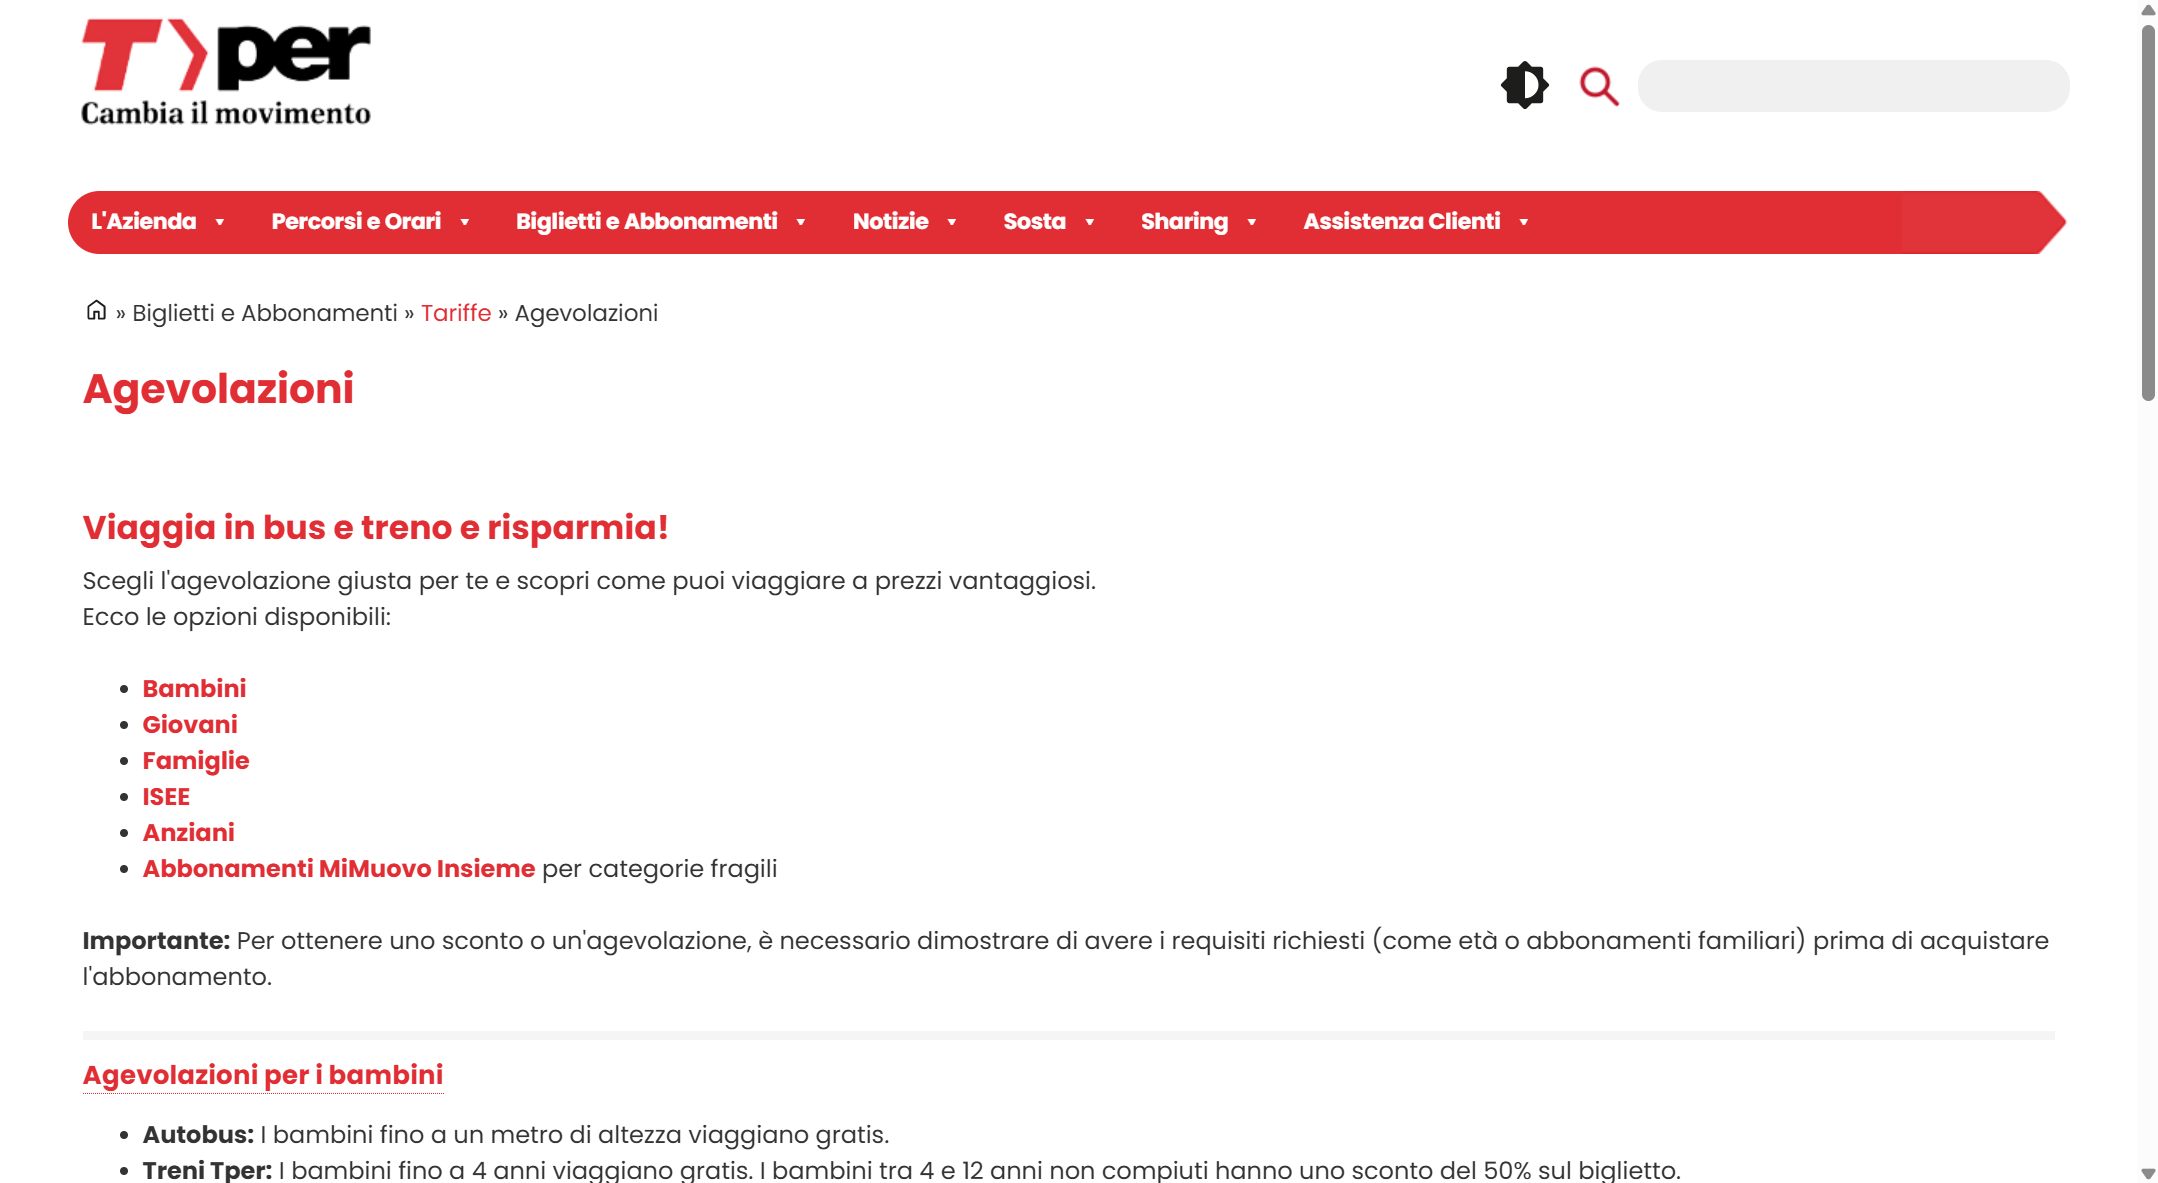
\includegraphics[width=0.85\textwidth]{Tper sito originale/Agevolazioni.png}
\par\small\textit{Before: original concessions page --- bureaucratic language, no guidance}
\vspace{0.4cm}
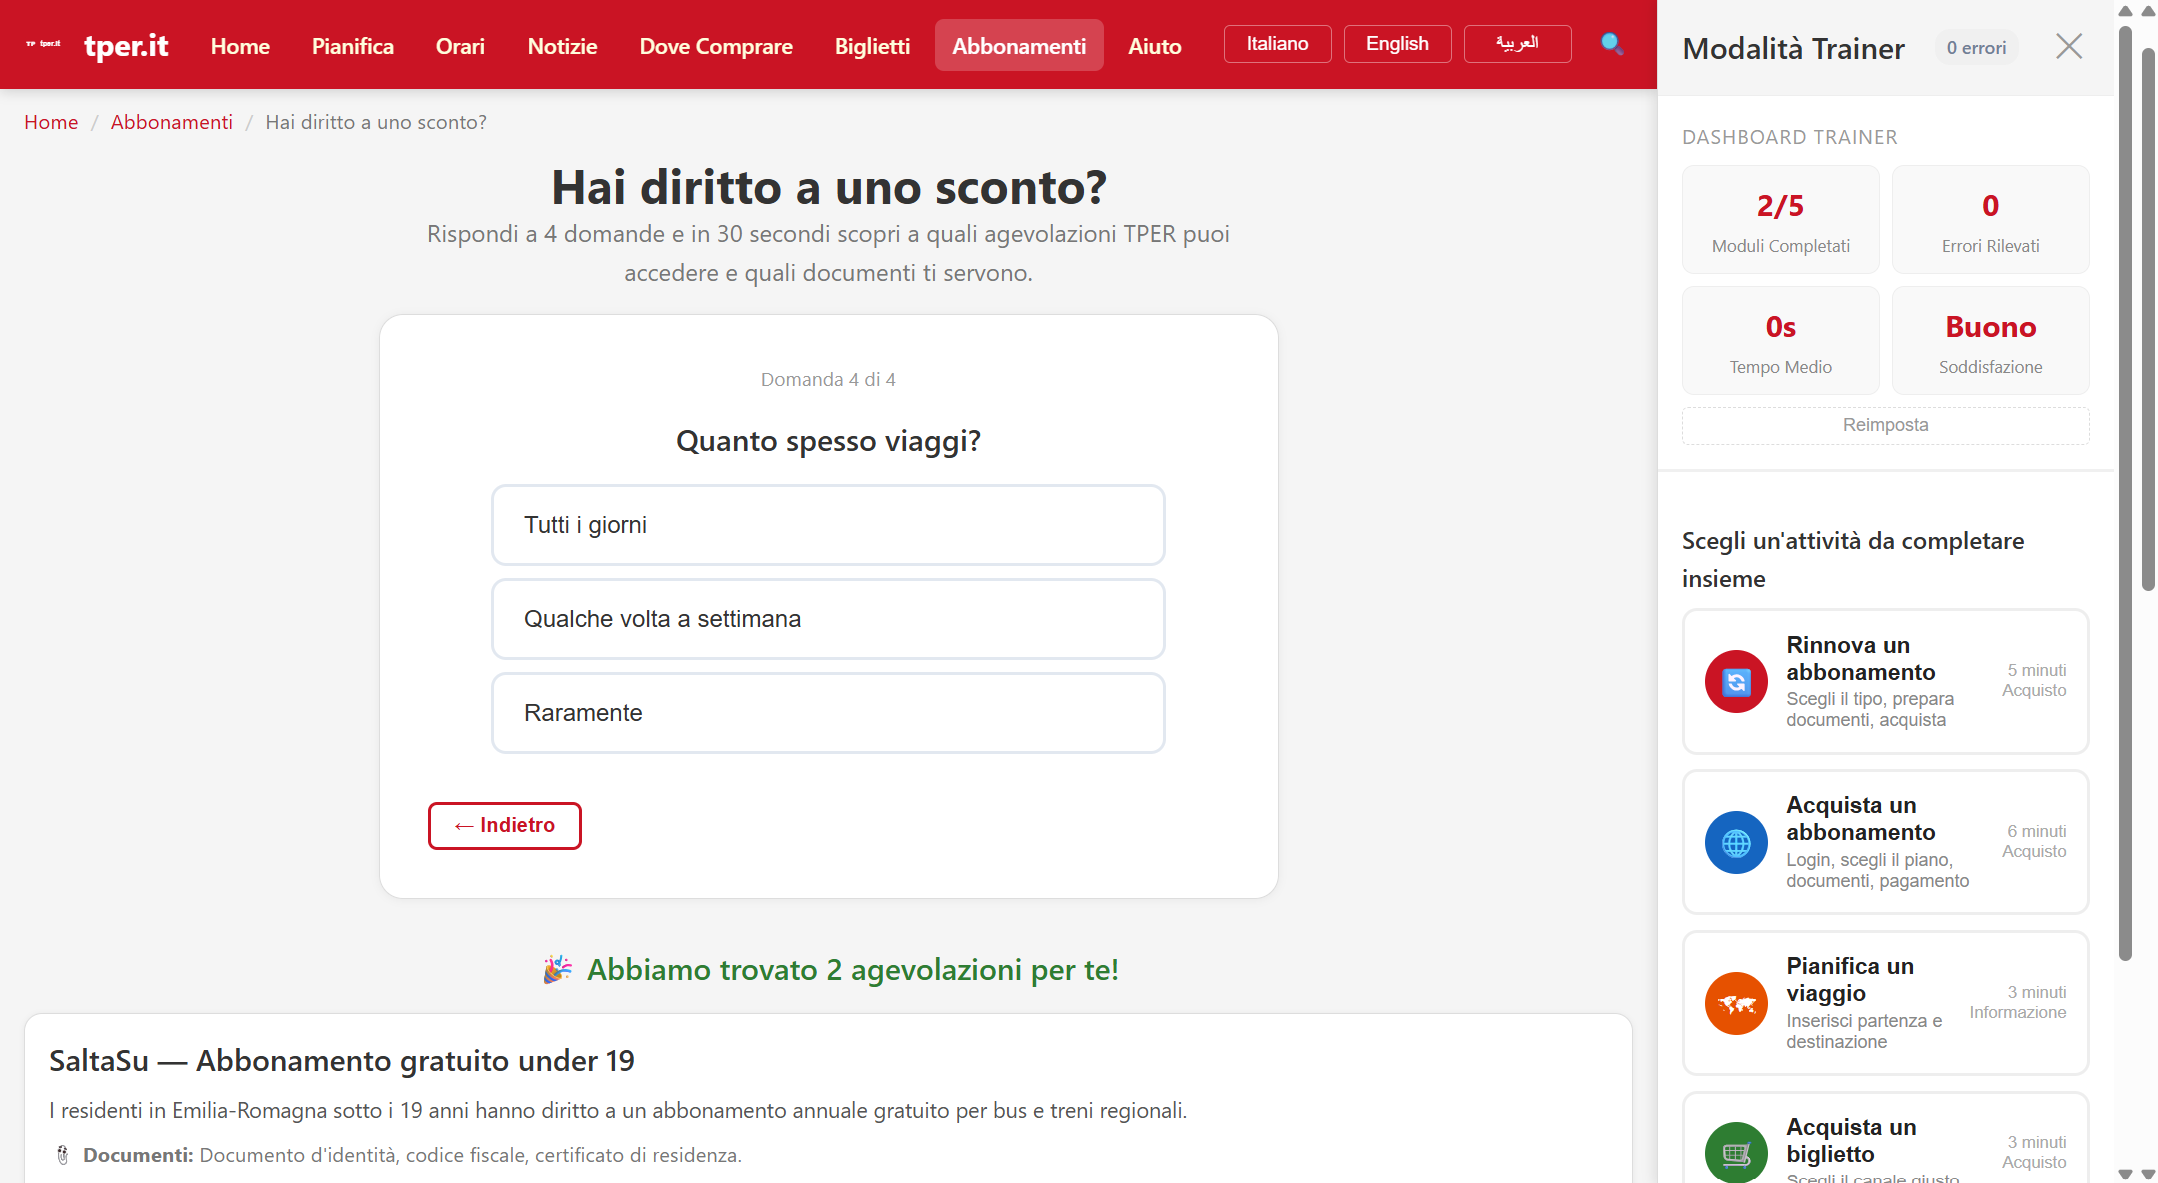
\includegraphics[width=0.85\textwidth]{Redesign Tper 2.0/Agevolazioni.png}
\par\small\textit{After: concessions wizard 2.0 --- 4 questions, personalised results, ISEE tooltip}
\caption{Concessions and Discounts}
\label{fig:comparison-agevolazioni}
\end{figure}

\begin{table}[H]
\centering
\small
\renewcommand{\arraystretch}{1.4}
\begin{tabular}{|p{0.5cm}|p{7cm}|p{7cm}|}
\hline
& \textbf{Before} & \textbf{After} \\ \hline
\cellcolor{primaryColor!15} &
\textit{Original concessions section} &
\textit{Concessions wizard in tper 2.0} \\ \hline

\raisebox{0.5cm}{\rotatebox{90}{\textbf{Access}}} &
Section buried 3+ levels deep in the navigation. Only reachable through ``Subscriptions'' $\rightarrow$ ``Carta Agevolata''. No direct path from the homepage (D2, UR-05). &
\textbf{Dedicated ``Am I entitled to a discount?'' path} visible from the homepage (``Discover Subscriptions'' card) and from the Subscriptions page with a prominent callout ``Find out in 30 seconds which discounts you can access''. Breadcrumb: Home $\rightarrow$ Subscriptions $\rightarrow$ Concessions (R2, R9). \\ \hline

\raisebox{0.5cm}{\rotatebox{90}{\textbf{Language}}} &
Bureaucratic register: ``ISEE'', ``DSU'', ``Carta Agevolata'', ``brackets'', ``resolutions''. No explanation of terms. For a foreign user (David Carter, language competence 2/5), terms remain incomprehensible even with Google Translate (UR-05, Use Case \#2). &
\textbf{Citizen-friendly language} with explanatory tooltips. On hover over ``ISEE'' it shows ``Indicatore della Situazione Economica Equivalente. Certifies the household income. Obtainable free of charge at CAF or online at INPS.'' Same approach for ``DSU'' and ``Carta Agevolata''. Available in IT/EN/AR (R9, R12). \\ \hline

\raisebox{0.5cm}{\rotatebox{90}{\textbf{Wizard}}} &
\textbf{Absent.} The user must read pages of resolutions and brackets to discover if they are entitled to a discount. No interactive guidance. David Carter's test shows 15 minutes of attempts followed by abandonment (Use Case \#2). &
\textbf{4-question wizard}: (1) How old are you? (2) Do you have an ISEE? (3) How often do you use public transport? (4) Who is the subscription for? Each answer filters available discounts in real time. Result: ``We found X discounts for you!'' with name, description, required documents, and direct link (RF-35, R9). \\ \hline

\raisebox{0.5cm}{\rotatebox{90}{\textbf{Documents}}} &
No preventive checklist. Required documents (ISEE, DSU, passport photo, ID) mentioned on separate bureaucratic pages. The user arrives at the counter without the right documents (Roberto, Use Case \#1). &
\textbf{Integrated document checklist} in the wizard results: each discount shows exactly which documents are needed, with tooltips on where to obtain them. Visual document reproduction (e.g. ``ISEE --- first page'' with yellow highlight of the value). ``View Subscriptions'' link to proceed with purchase (R11). \\ \hline

\raisebox{0.5cm}{\rotatebox{90}{\textbf{Impact}}} &
David Carter (Phase A): 3 months paying 50\euro/month instead of 30\euro. Roberto: arrives at the counter without documents and postpones. Average SUS 37.5/100. &
Laura P. (Phase D, T4): from 195\,s and 7 errors to 57\,s and 0 errors. Concessions wizard completed in 30 seconds. ISEE tooltip used spontaneously. SUS 72.5 (+35 points). \\ \hline
\end{tabular}
\caption{Concessions and Discounts}
\label{tab:comparison-agevolazioni}
\end{table}

\vspace{0.3cm}

% ============================================================
% COMPARISON 5: TRIP PLANNING
% ============================================================
\section{Trip Planning}
\label{sec:comparison-planning}

\textbf{D2 $\rightarrow$ R1+R2} --- Route planner on a separate page, reachable via the ``Routes and Timetables'' link on the homepage (1 click), but with no search fields visible directly on the homepage $\rightarrow$ Hero search + dedicated page. Maria: 724\,s, 16 errors, 19 backtracks on T2 (Phase A).

\begin{figure}[H]
\centering
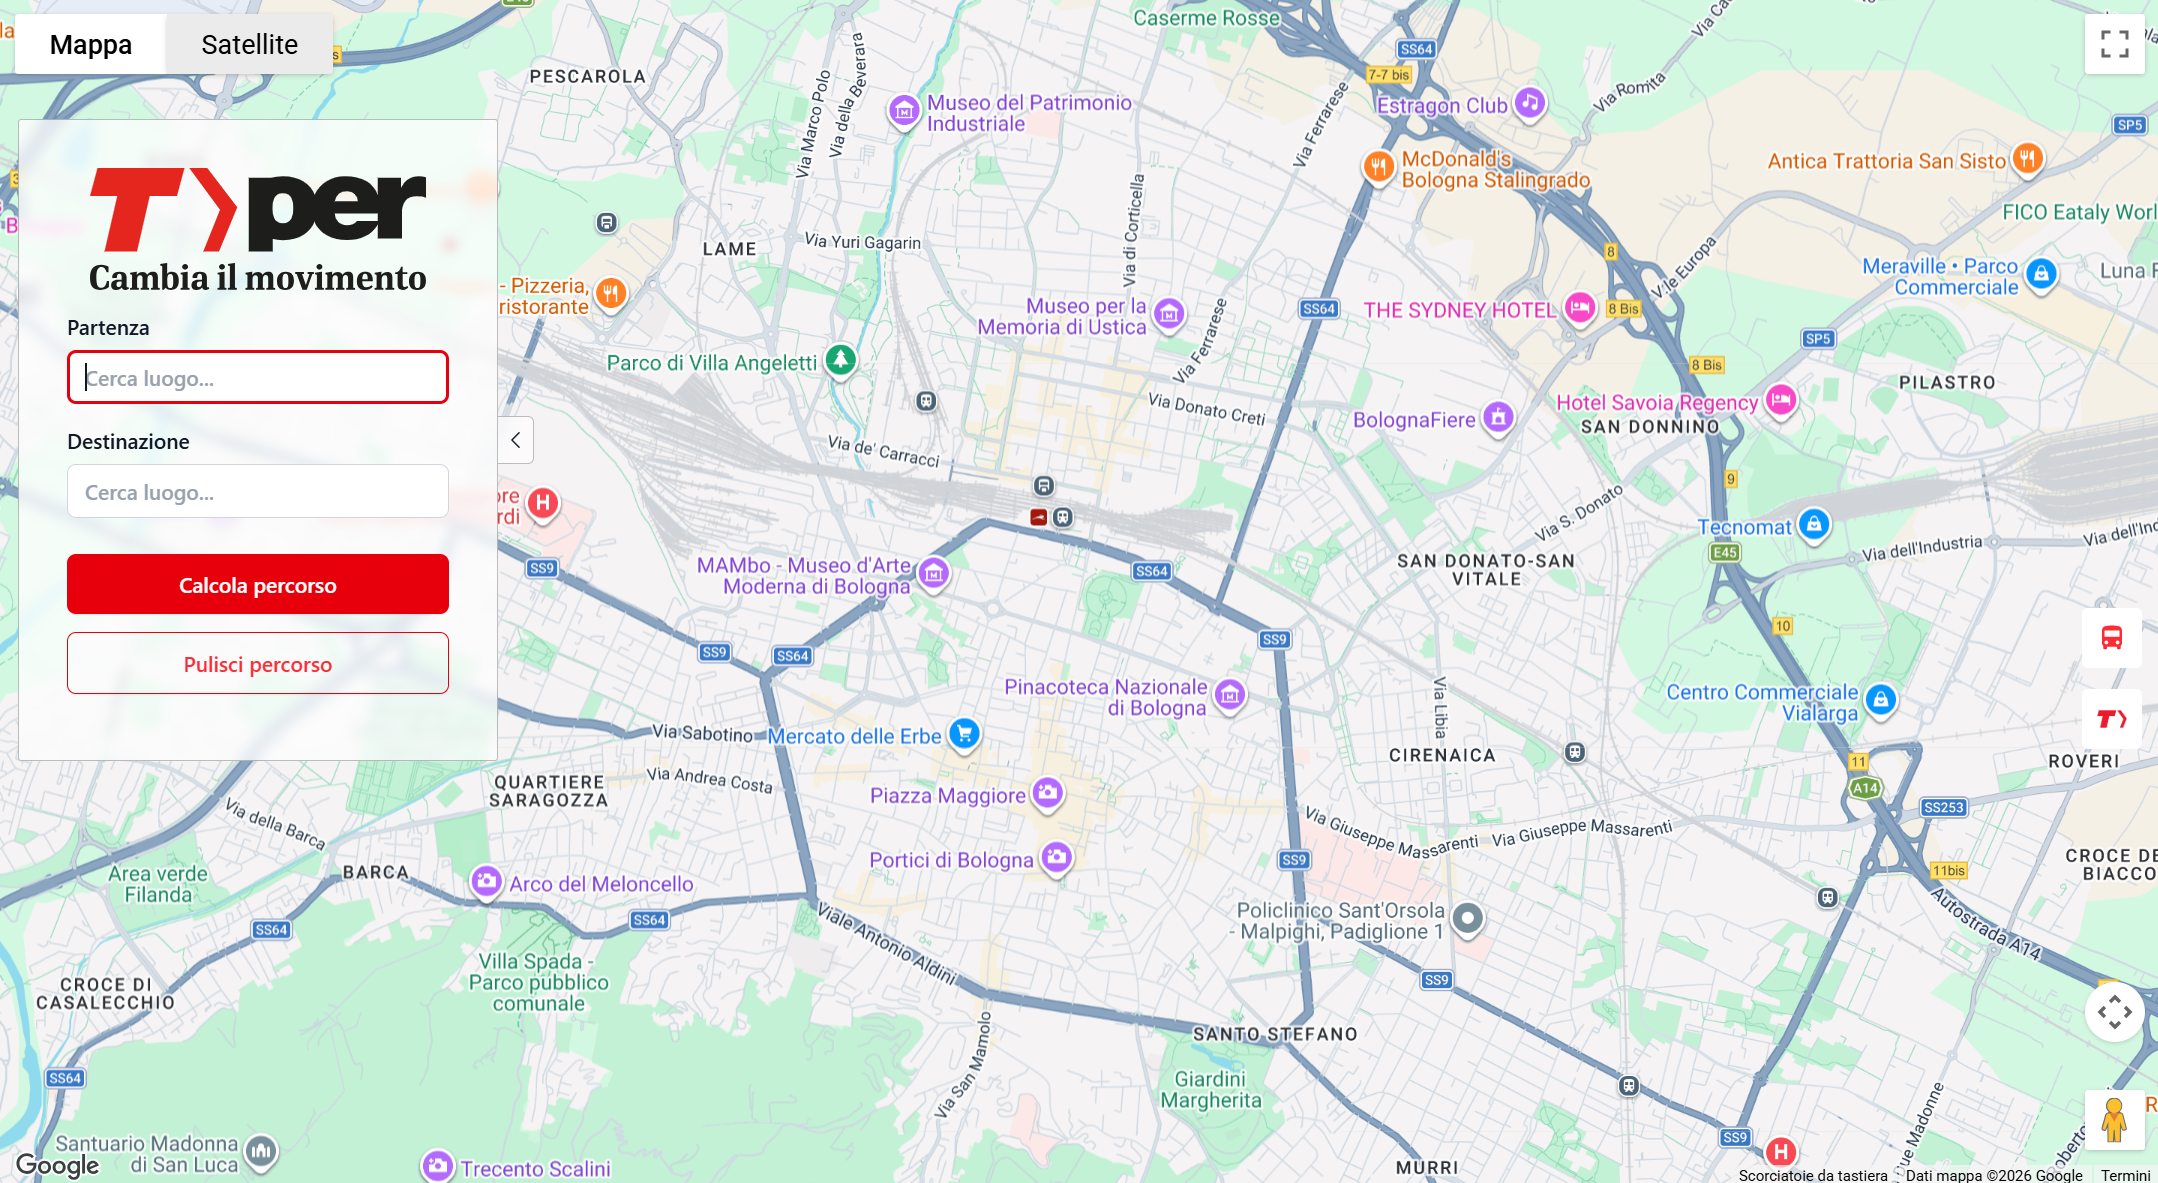
\includegraphics[width=0.85\textwidth]{Tper sito originale/Percorsi.png}
\par\small\textit{Before: original planner --- reachable from the homepage via ``Routes and Timetables'' (homepage link) $\rightarrow$ ``Calculate your route''}
\vspace{0.4cm}
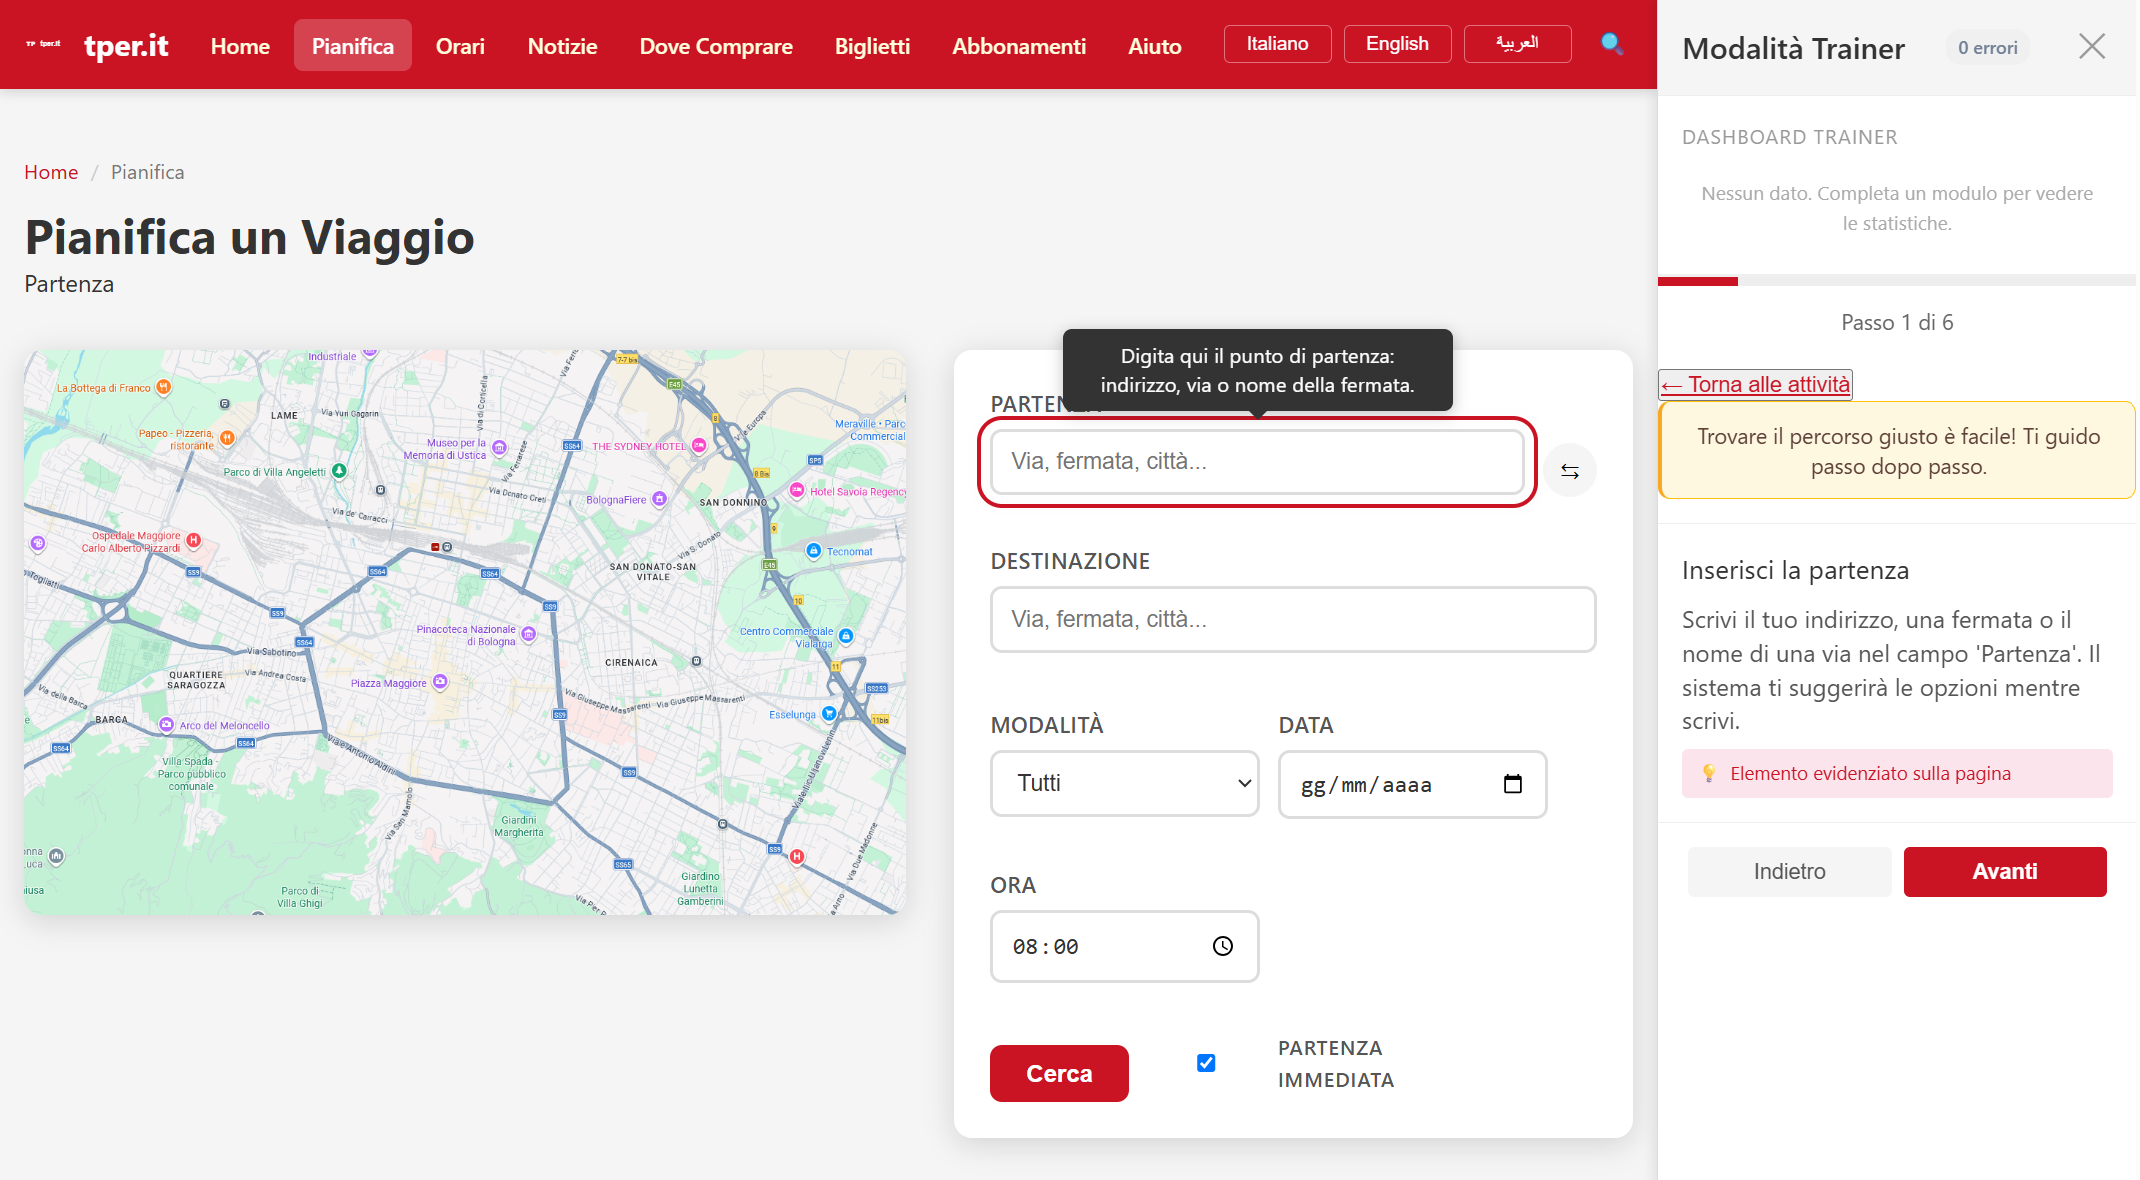
\includegraphics[width=0.85\textwidth]{Redesign Tper 2.0/Percorsi.png}
\par\small\textit{After: trip planner 2.0 --- hero search on homepage + dedicated page with map and form}
\caption{Trip Planning}
\label{fig:comparison-planning}
\end{figure}

\begin{table}[H]
\centering
\small
\renewcommand{\arraystretch}{1.4}
\begin{tabular}{|p{0.5cm}|p{7cm}|p{7cm}|}
\hline
& \textbf{Before} & \textbf{After} \\ \hline
\cellcolor{primaryColor!15} &
\textit{Original \texttt{tper.it} route planner} &
\textit{Trip planning in tper 2.0} \\ \hline

\raisebox{0.5cm}{\rotatebox{90}{\textbf{Access}}} &
``Routes and Timetables'' link visible on the homepage (1 click), leading to the planner page. No search fields visible directly on the homepage. The user must recognise the corporate label ``Routes and Timetables'' to start the task (D3). &
\textbf{Hero search on homepage}: ``From'' and ``To'' fields visible with no clicks needed. ``Plan'' section in main navigation (1 click). ``Plan'' card in the ``What do you want to do?'' grid with distinctive icon (R1, R2). \\ \hline

\raisebox{0.5cm}{\rotatebox{90}{\textbf{Form}}} &
Text search form with no suggestions. Single combined from/to field. No transport mode filter. No interactive map. &
\textbf{Full form}: separate from/to fields with swap button. Transport modes (bus/train/bike/walk). Date and time with ``Depart now'' checkbox. Interactive Bologna map alongside (click to enlarge). Autocomplete on fields (R1). \\ \hline

\raisebox{0.5cm}{\rotatebox{90}{\textbf{Results}}} &
Text list of results without timetables or duration. No price indication. No link to purchase channel. The user must take notes and search elsewhere for how to buy the ticket (UR-01, UR-03). &
\textbf{Structured results} with timetables, duration, and informative price for each option. ``Where to Buy'' link integrated in each result. Map/list toggle. Informational banner: ``On tper.it you cannot purchase --- find out how and where to buy'' (R1, R6). \\ \hline

\raisebox{0.5cm}{\rotatebox{90}{\textbf{Impact}}} &
Maria B. (Phase A): 724\,s, 16 errors, 19 backtracks. Cannot find the planner and gives up after 12 minutes. Average SUS 37.5/100. &
Laura P. (Phase D, T2): 115\,s, 1 error, 0 backtracks. ``Plan'' card recognised immediately. Hero search used without hesitation. SUS 72.5 (+35 points). \\ \hline
\end{tabular}
\caption{Trip Planning}
\label{tab:comparison-planning}
\end{table}

\vspace{0.3cm}

% ============================================================
% COMPARISON 6: TRAINER MODE AND SUPPORT
% ============================================================
\section{Trainer Mode and Support}
\label{sec:comparison-trainer}

\textbf{R5 $\rightarrow$ R4+R5+R6} --- No trainer $\rightarrow$ Sidebar 22 pages, 5 modules, operator script. Maria 0/5 tasks, SUS 27.5.

\begin{figure}[H]
\centering
\fcolorbox{borderColor}{backgroundColor}{%
\begin{minipage}{0.78\textwidth}
\centering
\vspace{1.5cm}
{\large\sffamily\textcolor{secondaryColor}{No Trainer Mode}}\\[4pt]
\small\textit{The original site offered no assisted mode whatsoever.}
\vspace{1.5cm}
\end{minipage}}
\par\small\textit{Before: no trainer mode --- only telephone help desk}
\vspace{0.4cm}
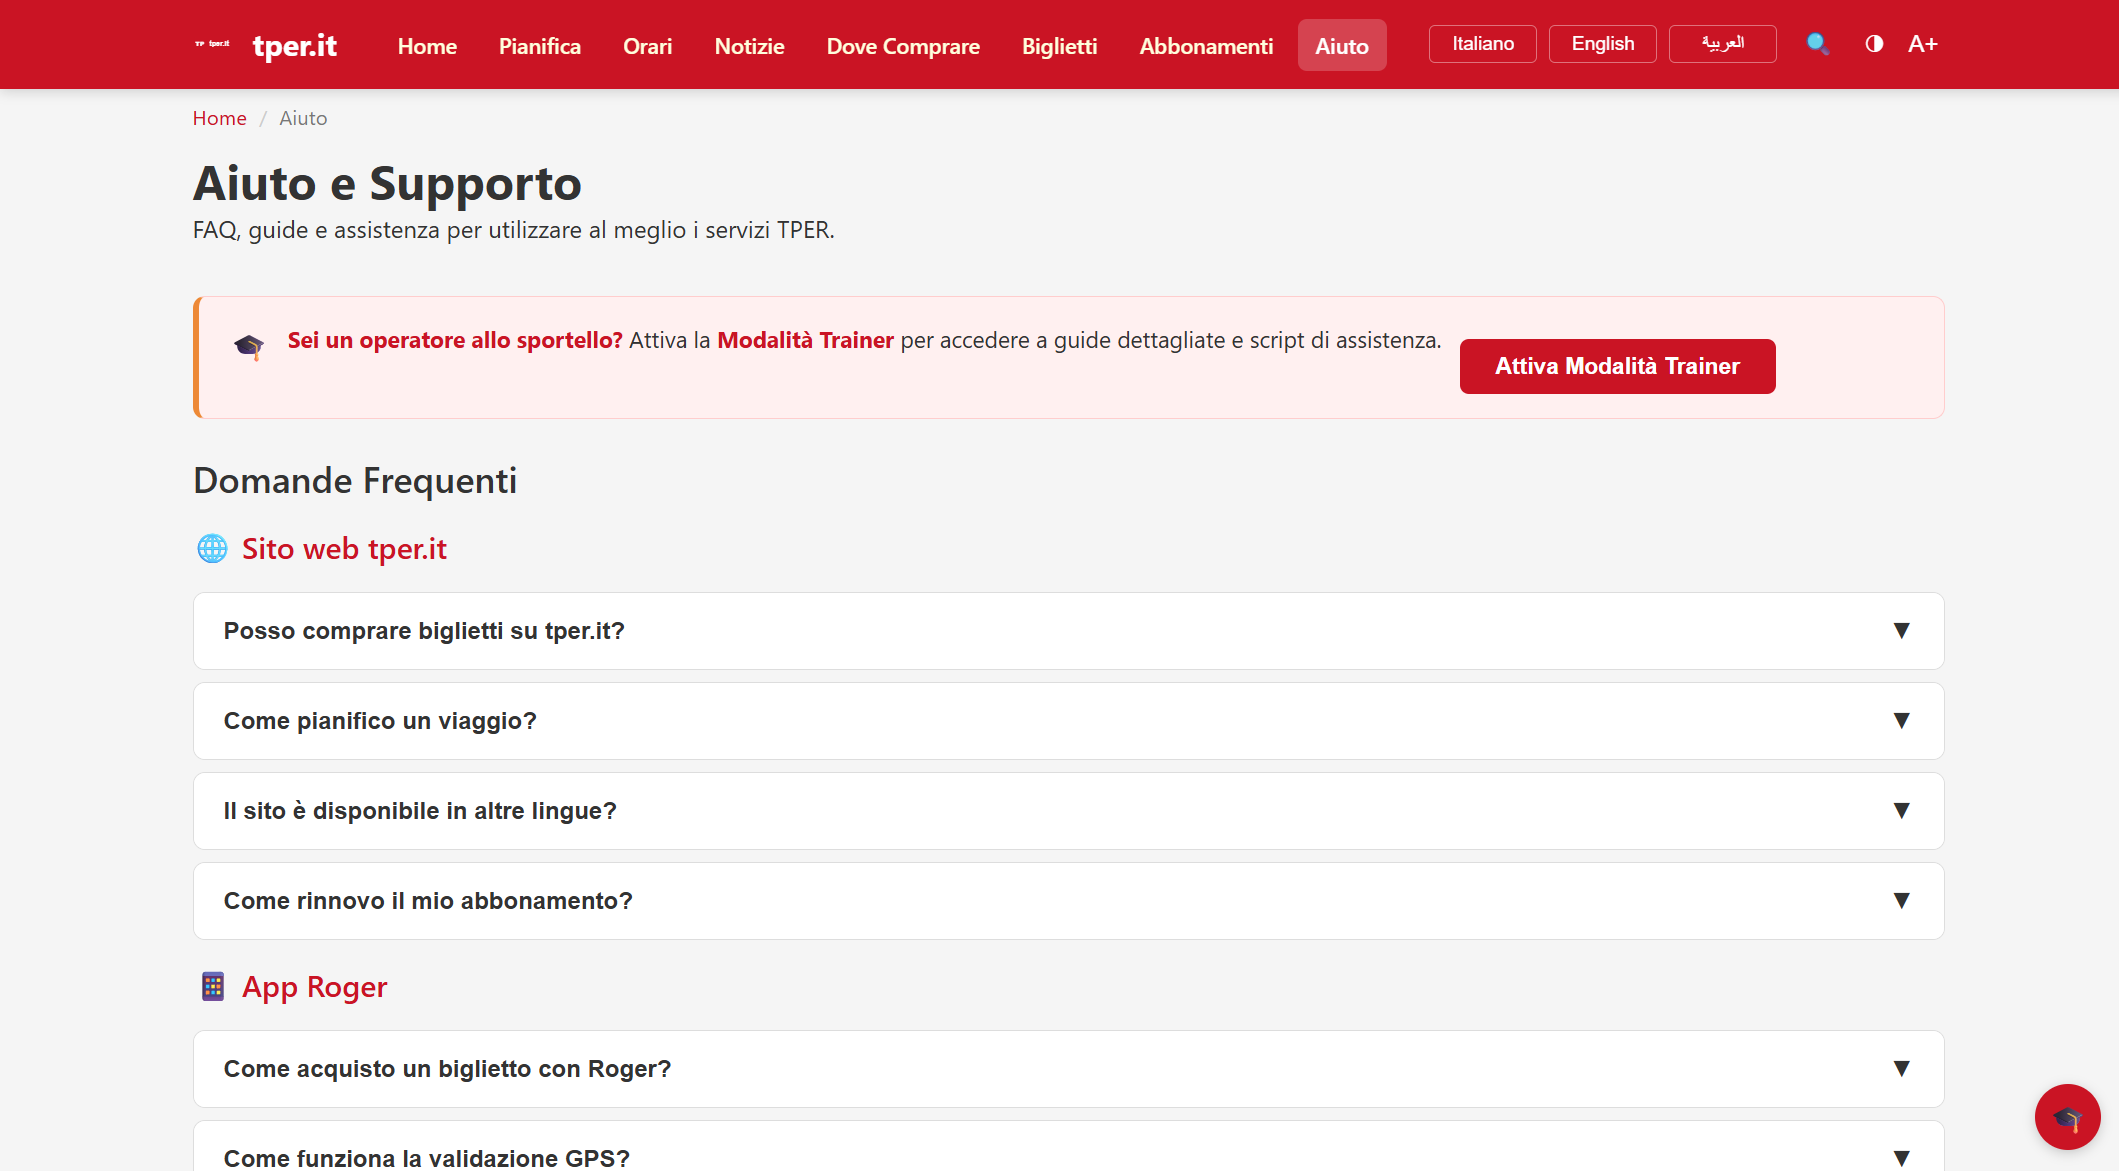
\includegraphics[width=0.85\textwidth]{Redesign Tper 2.0/Aiuto.png}
\par\small\textit{After: Help section with trainer mode, FAQ, step-by-step guides}
\caption{Trainer Mode and Support}
\label{fig:comparison-trainer}
\end{figure}

\begin{table}[H]
\centering
\small
\renewcommand{\arraystretch}{1.4}
\begin{tabular}{|p{0.5cm}|p{7cm}|p{7cm}|}
\hline
& \textbf{Before} & \textbf{After} \\ \hline
\cellcolor{primaryColor!15} &
\textit{Current support on \texttt{tper.it}} &
\textit{Trainer mode and support in tper 2.0} \\ \hline

\raisebox{0.5cm}{\rotatebox{90}{\textbf{Trainer}}} &
\textbf{Non-existent.} No assisted mode for counter operators. No step-by-step guidance mechanism to accompany users with low digital competence in navigating between channels. The only support channel is customer service (phone or email) (R4, R5). &
\textbf{Integrated sidebar} on all 22 pages of the site. 5 trainer modules: Renew, Purchase, Trip, Ticket, Top-up. Each module automatically loads the correct page with highlights on relevant elements. Activation: on request ($\mathcal{T}$ button) (R4, R5). \\ \hline

\raisebox{0.5cm}{\rotatebox{90}{\textbf{Script}}} &
No operational script for counter staff. &
5-step script for operators: (1) Identify the need, (2) Recommend the travel pass, (3) Direct to the correct channel, (4) Explain validation, (5) Confirm and ask if they need anything else (R4). \\ \hline

\raisebox{0.5cm}{\rotatebox{90}{\textbf{FAQ}}} &
Only help desk as a support channel. No interactive guidance, no organised FAQ (R10). &
\textbf{Accordion FAQ grouped by channel}: \texttt{tper.it}, Roger App, Punti Tper and Retailers, Fines, Contactless Onboard. Each section answers the most common questions for that channel. Includes direct links (e.g. from solweb FAQ $\rightarrow$ purchase page) (R9, R10). \\ \hline

\raisebox{0.5cm}{\rotatebox{90}{\textbf{Guides}}} &
Absent. &
3 step-by-step guide cards in the Help section: ``How to purchase on solweb'', ``How to use the Roger App'', ``How to find a Punto Tper''. Each with a direct CTA to the corresponding channel. Interactive wizards on Where to Buy, Tickets, and Subscriptions (R9). \\ \hline

\raisebox{0.5cm}{\rotatebox{90}{\textbf{Persistence}}} &
No session memory. If the user closes the browser or the timeout expires, they lose everything and must start over from scratch. &
\textbf{Auto-save} of the trainer session state in localStorage. The user can resume from the exact point where they left off. Printable summary with annotated screenshots and navigation path (R5, R6). \\ \hline
\end{tabular}
\caption{Trainer Mode and Support}
\label{tab:comparison-trainer}
\end{table}

\vspace{0.3cm}

% ============================================================
% COMPARISON 7: ACCESSIBILITY AND MULTILINGUAL
% ============================================================
\section{Accessibility and Multilingual Support}
\label{sec:comparison-a11y}

\textbf{R3+D3 $\rightarrow$ R8+R12} --- IT only, 10pt, <44px targets $\rightarrow$ IT/EN/AR, 14pt, WCAG AA. Chris 3/5 failed due to language.

\begin{table}[H]
\centering
\small
\renewcommand{\arraystretch}{1.4}
\begin{tabular}{|p{0.5cm}|p{7cm}|p{7cm}|}
\hline
& \textbf{Before} & \textbf{After} \\ \hline
\cellcolor{primaryColor!15} &
\textit{Current state of the \texttt{tper.it} live site} &
\textit{Accessibility and languages in tper 2.0} \\ \hline

\raisebox{0.5cm}{\rotatebox{90}{\textbf{Language}}} &
\textbf{Italian only.} No language selector, no content in English or Arabic. Foreign users completely excluded from online information services. Chris H. (English): 3/5 tasks failed despite high digital competence (R12). &
\textbf{IT + EN + AR.} Three-button language switcher always visible in the header of every page. Complete translation of labels, informational content, FAQ, and wizards. 1,600+ i18n keys in JavaScript files. RTL support for Arabic (R12). \\ \hline

\raisebox{0.5cm}{\rotatebox{90}{\textbf{Font Size}}} &
Small text (10--11pt). Reading difficulty for users over 65, particularly critical for channel names and tariffs. Maria B. could not distinguish buttons from static text (R8). &
\textbf{Minimum 14pt} on all text. \textbf{A+} button in header to further enlarge text with one click. Persistent toggle across pages (R8). \\ \hline

\raisebox{0.5cm}{\rotatebox{90}{\textbf{Contrast}}} &
Contrast not declared, likely below WCAG AA standard for some colour combinations. &
\textbf{Minimum 4.5:1 ratio} (WCAG AA). \textbf{$\blacksquare$} button to toggle high-contrast mode on all pages. Persistent toggle. Completely revised palette in high-contrast mode (R8). \\ \hline


\raisebox{0.5cm}{\rotatebox{90}{\textbf{Touch Targets}}} &
Touch targets below 44$\times$44px in many areas, making smartphone use difficult for users with reduced dexterity. &
\textbf{All interactive targets $\ge$ 44$\times$44px} (WCAG 2.1). Buttons, links, checkboxes, and radio buttons sized for error-free tactile interaction (R8). \\ \hline
\end{tabular}
\caption{Accessibility and Multilingual Support}
\label{tab:comparison-a11y}
\end{table}

\vspace{0.3cm}

% ============================================================
% COMPARISON 8: TONE AND TERMINOLOGY
% ============================================================
\section{Tone and Terminology}
\label{sec:comparison-tone}

\textbf{D3 $\rightarrow$ R9} --- Corporate terminology $\rightarrow$ User language + glosses. ``MiMuovo'', ``Sales Network'' incomprehensible to all.

\begin{table}[H]
\centering
\small
\renewcommand{\arraystretch}{1.4}
\begin{tabular}{|p{0.5cm}|p{7cm}|p{7cm}|}
\hline
& \textbf{Before} & \textbf{After} \\ \hline
\cellcolor{primaryColor!15} &
\textit{Current language on \texttt{tper.it}} &
\textit{Tone and terminology in tper 2.0} \\ \hline

\raisebox{0.5cm}{\rotatebox{90}{\textbf{Tone}}} &
Bureaucratic and institutional. Impersonal phrases, public administration lexicon. Cold and generic error messages. The user feels like an ``applicant'' rather than a customer (Issue D3). &
Encouraging and inclusive. First-person plural language: ``We'll help you choose'', ``No problem, we can try again together''. Error messages with a human tone and way out: ``Didn't find what you were looking for? Try one of these alternatives'' (R9). \\ \hline

\raisebox{0.5cm}{\rotatebox{90}{\textbf{Terms}}} &
Exclusively corporate terminology: \textit{Sales Network}, \textit{Automatic Issuing Machines}, \textit{MiMuovo}, \textit{SaltaSu}, \textit{Prontobus}, \textit{Discobus}. \texttt{solweb} and \textit{Roger} never explained or introduced. The user must know TPER jargon before using the site (Issue D3). &
\textbf{User-centric terminology with glosses}: ``Where to Buy'' (not ``Sales Network''), ``Online Subscriptions (solweb)'', ``Digital Tickets (Roger)'', ``Tobacconists and PuntoLis''. Every technical term is accompanied by an inline explanation or a tooltip on first use. The corporate name remains in parentheses for reference (R2, R9). \\ \hline

\raisebox{0.5cm}{\rotatebox{90}{\textbf{Messages}}} &
Impersonal system messages with no guidance. ``Error --- try again'' without explanation of cause or solution. The user abandons the flow (Issue D4). &
\textbf{Exponential messages} (R10): what happened, why it happened, how to fix it, what to do as an alternative. Contrast-background box with warning icon, positioned inline above the affected field. Micro-reinforcements after each step: ``Perfect, that's done!'' (R9). \\ \hline

\raisebox{0.5cm}{\rotatebox{90}{\textbf{Onboarding}}} &
No first-access path. The user lands on the homepage and must figure everything out alone. Maria B.: \textit{``I don't even know where to start''}. &
\textbf{``First Time'' Tour}: 4 illustrated screens explaining channels through everyday metaphors. Activatable from the Help button. Reassuring language: ``Don't worry, I'll show you where to go'' (R9). \\ \hline
\end{tabular}
\caption{Tone and Terminology}
\label{tab:comparison-tone}
\end{table}




